\documentclass{article}

% NeurIPS 2026 submission style. Do not use [preprint] or [final] for an
% anonymized conference submission.
\usepackage{neurips_2026}

\usepackage[utf8]{inputenc}
\usepackage[T1]{fontenc}
\usepackage{amsmath, amssymb, amsfonts}
\usepackage{booktabs}
\usepackage{graphicx}
\usepackage{multirow}
\usepackage{hyperref}
\usepackage{url}
\usepackage{xcolor}
\usepackage{enumitem}
\usepackage{nicefrac}
\usepackage{microtype}

\newcommand{\method}{Causal Response Evaluation}
\newcommand{\rir}{Randomized Intervention-Response Regularization}
\newcommand{\ire}{\ensuremath{\mathrm{IRE}}}
\newcommand{\mpd}{\ensuremath{\mathrm{MPD}}}
\newcommand{\csr}{\ensuremath{\mathrm{CSR}}}
\newcommand{\dr}{\ensuremath{\mathrm{DR}}}

\title{
Low Error, Wrong Response: \\
Causal Blindness in Multivariate Time-Series Forecasting
}

\author{
Anonymous Authors
}

\begin{document}
\maketitle

\begin{abstract}
Multivariate time-series forecasting models are usually selected by observational
errors such as MSE and MAE. This practice assumes that accurate prediction implies
that the model has learned useful temporal and cross-channel dependencies. We show
that this assumption can fail in a controlled but revealing way. We identify
\emph{causal blindness}: a forecaster can obtain low observational error while
producing an almost zero response to an intervention on the true driver of the
target. We construct a multivariate forecasting benchmark with one cause, one target,
and nineteen distractors, where the mechanism is $Y_t = 2C_{t-1}+\epsilon_t$ and the
horizon-1 counterfactual response is analytically known. Across DLinear, PatchTST,
iTransformer, Crossformer, TimeMixer, and DUET, a standardized intervention whose
expected response is about $5.0$ often yields predicted responses close to zero,
despite strong sensitivity to the target's own history. We introduce
intervention-aware diagnostics, including interventional response error and response
slope. A functional sensitivity analysis shows that the learned predictors are
locally far more sensitive to target history than to the true last-step driver,
providing an operational explanation for the failure. We propose \rir{} (RIR), a
lightweight training objective that regularizes the forecast response to known
interventions. RIR repairs response curves for both iTransformer and DUET-Mix, and
an augmented ETTh1 diagnostic suggests that response alignment need not degrade the
ordinary MSE/MAE of original benchmark channels.
\end{abstract}

\section{Introduction}

Multivariate long-term time-series forecasting (MLTSF) has advanced rapidly through
architectures based on linear projections, patching, transformers, inverted
attention, cross-dimensional attention, decomposition, multiscale mixing, and
dual clustering
\citep{zeng2023transformers,nie2023patchtst,liu2024itransformer,zhang2023crossformer,wang2024timemixer,qiu2025duet}.
Despite architectural differences, most models are selected and compared using
observational forecasting errors such as MSE and MAE. This evaluation practice
implicitly assumes that if a model predicts a target well, then it has learned the
relevant temporal and cross-channel dependencies.

We argue that this assumption is incomplete. In many scientific, industrial, and
operational settings, a forecaster is not only expected to extrapolate smooth curves;
it is expected to respond correctly when a driver changes. For example, load should
respond to upstream temperature or demand changes, downstream traffic should respond
to upstream flow, and physical targets should respond to their known input drivers.
A model that obtains low MSE by relying on target autocorrelation may still be
unreliable under interventions, distribution shifts, or policy changes.

This paper studies the following question:

\begin{quote}
\emph{Do modern multivariate forecasters respond to the true causal driver when the
driver is intervened on?}
\end{quote}

We show that the answer can be no, even when the causal mechanism is simple and
analytically known. We construct a controlled benchmark with $N=21$ channels: one
cause $C$, one target $Y$, and nineteen distractors. The target is generated by
\begin{equation}
Y_t = 2 C_{t-1} + \epsilon_t,
\label{eq:structural}
\end{equation}
with small noise. Since the mechanism is known, changing the last historical cause
value has a known horizon-1 counterfactual effect on the target. This makes it
possible to evaluate not only whether forecasts are accurate, but whether their
\emph{response} to a cause intervention has the correct direction and magnitude.

Our empirical finding is striking. Across DLinear, PatchTST, iTransformer,
Crossformer, TimeMixer, and DUET, a standardized cause shift whose expected
horizon-1 target response is approximately $5.000$ leads to predicted changes near
zero. In particular, a strong DUET configuration obtains low target MSE but predicts
only $0.029$ for an intervention whose expected response is $5.000$. Meanwhile,
zeroing the target history substantially changes the forecasts for all models. In
other words, these models are not generally insensitive; rather, they are highly
sensitive to the target's own history and weakly sensitive to the true causal driver.

We call this failure mode \emph{causal blindness}. It differs from poor forecasting:
some affected models achieve low observational error. It also differs from generic
robustness failure: the problem is not merely that inputs are perturbed, but that
the model's response is misaligned with an analytically known mechanism.

\begin{figure}[t]
\centering
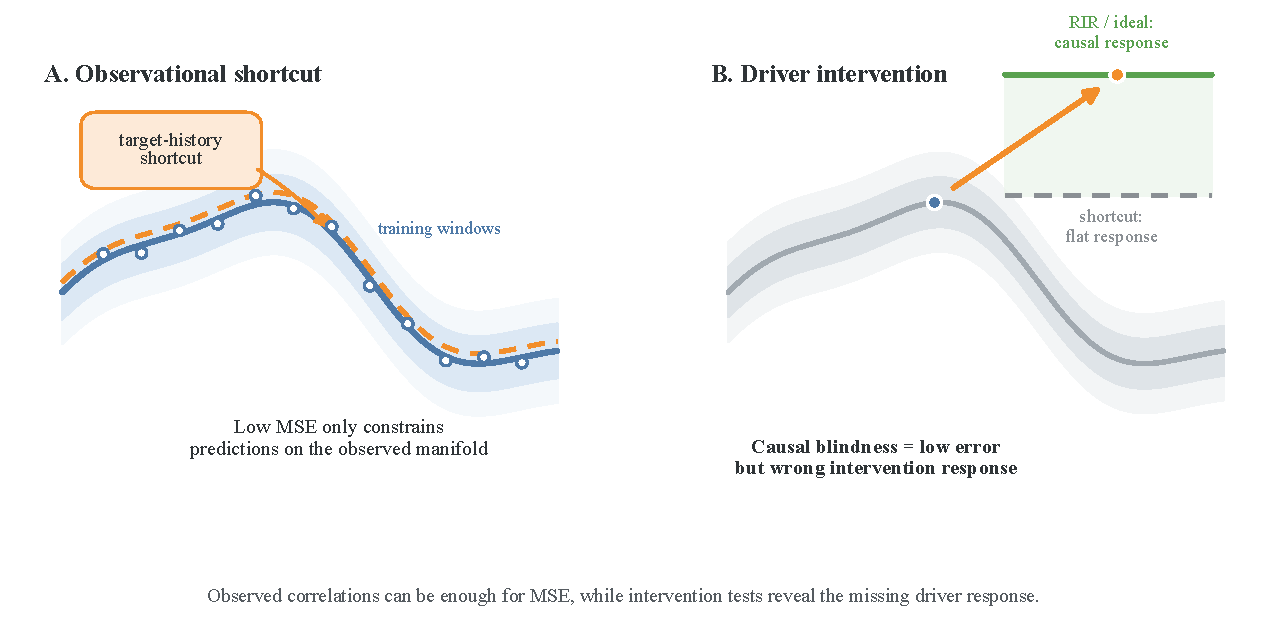
\includegraphics[width=\linewidth]{figures/concept_causal_blindness.pdf}
\caption{Causal blindness. Observational training can fit the data manifold with
low MSE by exploiting target-history shortcuts. When the true driver is intervened
on, the correct response moves off the observed manifold, but a shortcut forecaster
can remain almost unchanged.}
\label{fig:concept}
\end{figure}

Our contributions are:

\begin{itemize}[leftmargin=*]
    \item We formulate causal blindness as a hidden failure mode of MLTSF models:
    low observational forecasting error can coexist with near-zero response to the
    true causal driver.
    \item We construct a controlled multivariate forecasting benchmark with known
    horizon-1 counterfactual responses, enabling direct evaluation of response
    correctness rather than only prediction accuracy.
    \item We introduce intervention-aware diagnostics: cause sensitivity, distractor
    sensitivity, target-history sensitivity, horizon-1 interventional response
    error, response slope, and sign accuracy.
    \item We provide a functional sensitivity diagnosis showing that low-error
    predictors can be locally aligned with target-history shortcuts rather than the
    true driver; RIR changes this local response geometry.
    \item We provide evidence across five representative model families and a recent
    DUET baseline, showing that causal blindness is not restricted to a single
    architecture or to channel-independent modeling.
    \item We instantiate a simple remedy, \rir{}, that regularizes the response to
    randomized counterfactual interventions. RIR raises the predicted response from
    near zero to more than $80\%$ of the analytically expected effect on iTransformer
    and DUET-Mix, and it recovers near-linear response curves across positive and
    negative intervention magnitudes.
    \item We include an augmented ETTh1 diagnostic showing that response alignment
    improves a semi-synthetic causal target without degrading the MSE/MAE of the
    original \texttt{OT} channel across three seeds.
\end{itemize}

\section{Related Work}
\label{sec:related_main}

Modern MLTSF models include transformer-based sequence models
\citep{zhou2021informer,wu2021autoformer,zhou2022fedformer}, channel-independent
patch models \citep{nie2023patchtst}, linear baselines
\citep{zeng2023transformers}, inverted and cross-dimensional transformers
\citep{liu2024itransformer,zhang2023crossformer}, multiscale mixing
\citep{wang2024timemixer}, and dual clustering \citep{qiu2025duet}. These works
primarily optimize observational MSE/MAE. Our contribution is not another
forecasting backbone; it is an intervention-aware evaluation and training protocol
showing that cross-channel access does not imply correct causal response.

Our work connects to shortcut learning \citep{geirhos2020shortcut}, invariant and
causal representation learning
\citep{arjovsky2019invariant,scholkopf2021toward}, and classical intervention-based
causal reasoning \citep{granger1969investigating,pearl2009causality,peters2017elements}.
Recent forecasting work has begun to address causal evaluation and counterfactual
reasoning \citep{crasson2024training,yan2023self,yang2025learning}. We differ in
focus: rather than estimating treatment effects from observational regimes or
generating explanations, we test whether standard MLTSF predictors have the correct
numerical response to known driver interventions.

\section{Problem Setup and Evaluation Metrics}
\label{sec:evaluation}

Let $X_{1:T}\in\mathbb{R}^{T\times N}$ be a history window and
$Z_{T+1:T+H}\in\mathbb{R}^{H\times N}$ the full future window. A forecaster
$f_\theta$ is usually selected by observational error,
\begin{equation}
\mathcal{L}_{\mathrm{obs}}
=
\frac{1}{HN}\left\|f_\theta(X_{1:T})-Z_{T+1:T+H}\right\|_F^2 .
\end{equation}
We ask a different question: if a target channel $y$ is driven by a cause channel
$c$, does the horizon-1 prediction respond correctly when $c$ is intervened on?
For an intervention $a$, define
\begin{equation}
\Delta \hat{y}_{1}(a)=f_\theta(X^a)_{1,y}-f_\theta(X)_{1,y},\qquad
\Delta y_{1}(a)=Z^a_{1,y}-Z_{1,y}.
\end{equation}
We call a model \emph{causally blind} when it has low observational error but a
large response error $|\Delta\hat{y}_{1}(a)-\Delta y_{1}(a)|$ for a known driver
intervention.

\paragraph{Scope of causal evaluation.}
Unlike observational forecasting, interventional evaluation requires ground-truth
counterfactual responses. Standard benchmarks such as Traffic, Electricity, and
raw ETT provide observed futures but no \emph{do}-labels for channel
interventions, so raw benchmark accuracy alone is not causal evidence. We therefore
use settings where the response is known by construction: a controlled benchmark
for causal evidence and an augmented real-world benchmark for side-effect and
realism diagnostics.

\paragraph{Controlled benchmark.}
We construct a 21-channel benchmark with one cause $C$, one target $Y$, and
19 distractors. The structural equation is
\begin{equation}
Y_t=2C_{t-1}+\epsilon_t ,
\label{eq:main_structural}
\end{equation}
with small Gaussian noise. The input length and prediction length are both 96.
All channels are standardized once using training-set statistics; interventions are
then applied in standardized input space. The final channel order is
$C,D_1,\ldots,D_{19},Y$.

Our causal evaluation uses a last-step cause intervention,
\begin{equation}
C_T' = C_T+\delta,\qquad C_t'=C_t \ \mathrm{for}\ t<T .
\end{equation}
Since Eq.~\eqref{eq:main_structural} implies
$Y_{T+1}=2C_T+\epsilon_{T+1}$, the horizon-1 counterfactual response is exact and
does not require assumptions about future cause trajectories. In standardized
coordinates,
\begin{equation}
\Delta y^{\mathrm{std}}_{T+1}
=2\frac{\sigma_C}{\sigma_Y}\Delta C_T^{\mathrm{std}},
\end{equation}
and in our benchmark $2\sigma_C/\sigma_Y=1.000076888$, so $\delta=5$ implies an
expected response of $5.000384$. We report horizon-1 interventional response error
(\ire), response slope, and mean prediction difference (\mpd). Full metric
definitions, all-history sensitivity tests, and normalization caveats are in
Appendix~\ref{app:benchmark}.

\section{Causal Blindness: Diagnosis and Why it Happens}
\label{sec:blindness}

We evaluate DLinear, PatchTST, iTransformer, Crossformer, TimeMixer, and DUET.
The architectures span linear decomposition, channel-independent patching,
variable-token attention, cross-dimensional attention, multiscale mixing, and
dual temporal-channel clustering. Table~\ref{tab:main_failure} shows the central
failure: models with low target MSE can have almost zero response to the true
driver. TimeMixer has the lowest MSE among the Time-Series-Library models but
zero measured response; DUET-Mix also obtains low error while predicting only
$0.053$ for an expected response of $5.000$.

\begin{table}[t]
\centering
\caption{Main causal-blindness result. The expected horizon-1 response to
$C_T\leftarrow C_T+5$ is $5.000384$. ``Pred. $|\Delta|$'' reports the absolute
mean target response; slope is computed from signed responses.}
\label{tab:main_failure}
\resizebox{\linewidth}{!}{
\begin{tabular}{lrrrrrr}
\toprule
Model & Target MSE & Target MAE & Pred. $|\Delta|$ & H1 IRE & Slope & Target-zero MPD \\
\midrule
DLinear      & 0.5454 & 0.6220 & 0.000 & 5.000 & 0.000 & 0.648 \\
PatchTST     & 0.2960 & 0.4272 & 0.000 & 5.000 & 0.000 & 0.799 \\
iTransformer & 0.0608 & 0.1909 & 0.032 & 4.994 & 0.001 & 0.870 \\
Crossformer  & 0.0157 & 0.0994 & 0.001 & 5.000 & 0.000 & 0.884 \\
TimeMixer    & 0.0109 & 0.0831 & 0.000 & 5.000 & 0.000 & 0.838 \\
DUET-Mix     & 0.0245 & 0.1262 & 0.053 & 4.998 & 0.000 & 0.789 \\
\bottomrule
\end{tabular}
}
\end{table}

This result is not explained away by preprocessing. A correctly specified ARX
baseline using $C_T$ recovers a response slope of $0.9995$ under the same
standardization, while a target-only AR baseline remains non-responsive. Nor is the
effect only a large out-of-distribution shift: for
$\delta\in\{\pm0.1,\pm0.25,\pm0.5,\pm1\}$, iTransformer has small-delta slope
$-0.022$, PatchTST and TimeMixer have slope $0$, and ARX remains calibrated
($0.9995$). Table~\ref{tab:main_sanity} summarizes these checks. The ARX result is
important because it uses the same standardization and evaluation code as the deep
forecasters; therefore a near-zero response is not forced by the data pipeline. The
small-delta result is equally important because it shows that causal blindness is
already visible in the local perturbation regime, not only under the visually
striking $\delta=5$ intervention.
Appendix~\ref{app:lookback} further varies the look-back window for DUET-Mix and
finds near-zero response slopes from $T=48$ to $T=336$.

\begin{table}[t]
\centering
\caption{Sanity checks for the response evaluation. ARX confirms that the same
preprocessing and evaluation pipeline can recover the correct response. Small-delta
tests use $\delta\in\{\pm0.1,\pm0.25,\pm0.5,\pm1\}$ and show that near-zero
response is not merely a large-shift artifact.}
\label{tab:main_sanity}
\resizebox{\linewidth}{!}{
\begin{tabular}{llrrrr}
\toprule
Check & Model & H1/Target MSE & Small-delta slope & Full-sweep slope & Mean IRE \\
\midrule
Pipeline & AR($Y_T$) & 0.0183 & 0.0000 & 0.0000 & -- \\
Pipeline & ARX($C_T$) & 0.0010 & \textbf{0.9995} & \textbf{0.9995} & 0.0002 \\
Local response & iTransformer & 0.0608 & -0.0220 & -0.0008 & 0.4737 \\
Local response & PatchTST & 0.2960 & 0.0000 & 0.0000 & 0.4625 \\
Local response & TimeMixer & 0.0109 & 0.0000 & 0.0000 & 0.4625 \\
\bottomrule
\end{tabular}
}
\end{table}

The failure patterns are informative. Strict channel-independent predictors can be
structurally blind because the target prediction path cannot use another channel.
Channel-mixing models have access to the cause, but access is not alignment:
observational training can still favor target-history shortcuts. Crossformer also
responds more to distractor shifts than to the true cause in broad sensitivity
tests, suggesting that cross-channel interaction is not necessarily causal
interaction.

\paragraph{Why can low MSE coexist with wrong response?}

Observational error constrains a predictor's values on the observed data manifold,
but not its response to interventions. Suppose
$Y_{T+1}=g(C_T)+\epsilon$ and the target history $S=X_{1:T,Y}$ predicts the driver
well under the observational distribution: $C_T=q(S)+\nu$ with
$\mathbb{E}\nu^2\leq\eta^2$. If $g$ is $L$-Lipschitz, the shortcut
$h(S)=g(q(S))$ satisfies
\begin{equation}
\mathbb{E}\left(Y_{T+1}-h(S)\right)^2
\leq L^2\eta^2+\mathbb{E}\epsilon^2
\end{equation}
when the structural noise is mean-zero and independent of $\nu$. Thus a predictor
that ignores $C_T$ can be accurate whenever $S$ predicts $C_T$ on the training
manifold. Under the intervention $C_T\leftarrow C_T+\delta$, however, the shortcut
has zero response while the structural response is $g(C_T+\delta)-g(C_T)$.

We test this explanation directly using functional sensitivity. With
$\tau=0.05$, we measure
\begin{equation}
S(a)=
\mathbb{E}\left|
\frac{f_\theta(X+\tau a)_{1,Y}-f_\theta(X-\tau a)_{1,Y}}{2\tau}
\right|,
\end{equation}
where $a$ perturbs either the last cause value or the last target-history value.
Figure~\ref{fig:sensitivity} shows that MSE-trained models are locally much more
sensitive to target history than to the true last-step driver. RIR reverses this
imbalance for iTransformer.

\begin{figure}[t]
\centering
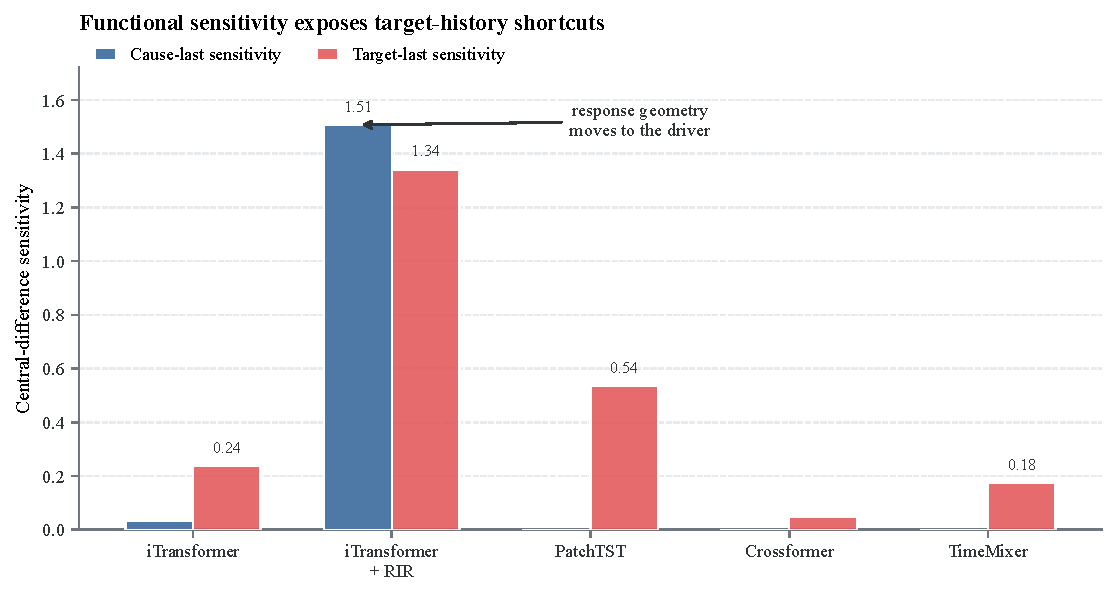
\includegraphics[width=\linewidth]{figures/functional_sensitivity_bars.pdf}
\caption{Functional input sensitivity of the horizon-1 target prediction,
measured by central differences with $\tau=0.05$. MSE-trained models are mostly
aligned with target-history shortcuts; RIR restores cause sensitivity.}
\label{fig:sensitivity}
\end{figure}

\section{Proposed Method: Randomized Intervention-Response Regularization}
\label{sec:rir}

RIR is a lightweight response-supervision objective for settings where domain
knowledge, a simulator, or benchmark construction provides a known driver and
horizon-1 response. During training, we sample
$\delta_i=s_i m_i$, where $s_i\in\{-1,1\}$ is uniform and
$m_i\sim\mathrm{Uniform}(\rho\Delta_{\max},\Delta_{\max})$. We intervene only on
the last historical driver value and define
$\Delta y_i^\star=(2\sigma_C/\sigma_Y)\delta_i$ for the synthetic benchmark. The
response loss is sliced to the horizon-1 target:
\begin{equation}
\mathcal{L}_{\mathrm{resp}}
=
\frac{1}{B}\sum_{i=1}^{B}
\left[
f_\theta(X_i^{\mathrm{cf}})_{1,Y}
-f_\theta(X_i)_{1,Y}
-\Delta y_i^\star
\right]^2 .
\end{equation}
To avoid indiscriminate reactivity, we also perturb last-step distractor values and
penalize target response:
\begin{equation}
\mathcal{L}_{\mathrm{dist}}
=
\frac{1}{B}\sum_{i=1}^{B}
\left[
f_\theta(X_i^{\mathrm{dist}})_{1,Y}
-f_\theta(X_i)_{1,Y}
\right]^2 .
\end{equation}
The training loss is
\begin{equation}
\mathcal{L}=\mathcal{L}_{\mathrm{pred}}
+\lambda_1\mathcal{L}_{\mathrm{resp}}
+\lambda_2\mathcal{L}_{\mathrm{dist}}.
\label{eq:main_rir}
\end{equation}
RIR adds no parameters, but uses three forward passes per step: original, causal
intervention, and distractor intervention.

\begin{figure}[t]
\centering
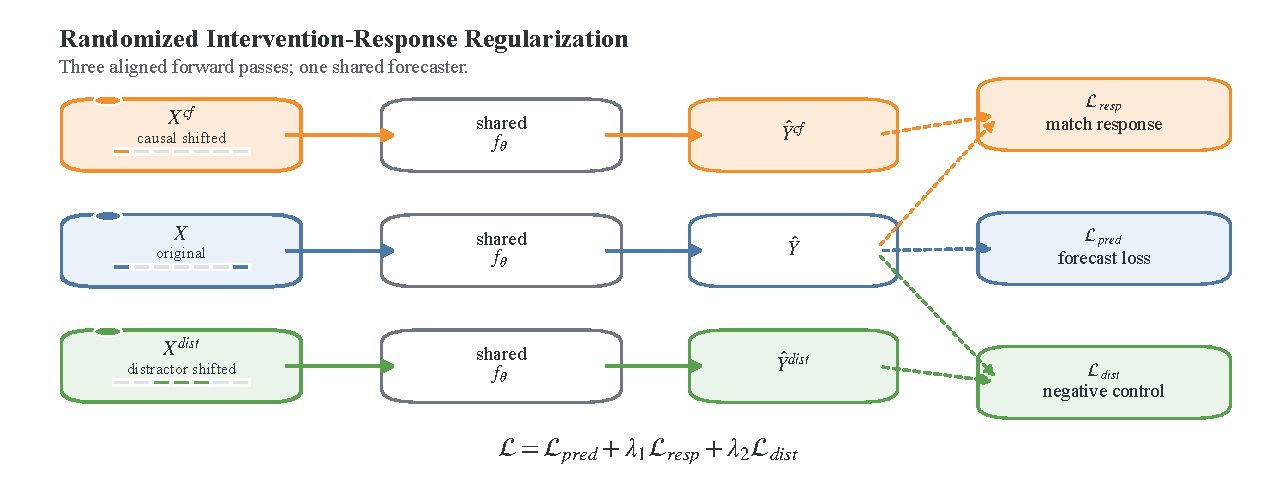
\includegraphics[width=\linewidth]{figures/rir_workflow.pdf}
\caption{RIR training workflow. The same forecaster is evaluated on the original
input, a last-step causal intervention, and a distractor intervention. The response
loss aligns the known driver response, while the distractor loss discourages
indiscriminate sensitivity.}
\label{fig:rir_workflow}
\end{figure}

\paragraph{What supervision does RIR require?}
RIR is not intended to replace causal discovery. It is useful when a practitioner
has a trusted response label for at least one driver-target pair, for example from a
physical simulator, a controlled intervention, an engineering specification, or a
benchmark construction. The label need not specify a full causal graph or every
future horizon. In our experiments, it specifies only the horizon-1 response of a
single target to a last-step driver intervention. This limited supervision is enough
to change the local response geometry of the forecaster. In domains where only
partial knowledge is available, the same objective can be applied sparsely: supervise
known driver-target pairs, leave unknown pairs unconstrained, and use distractor or
negative-control variables when domain knowledge indicates zero response.

\paragraph{Why include the distractor term?}
Without $\mathcal{L}_{\mathrm{dist}}$, response supervision can teach a model to be
reactive without teaching it where to be reactive. In our ablations
(Appendix~\ref{app:rir}), a response-only loss repairs the cause response but also
creates large false response to last-step distractor interventions. The distractor
term acts as a local negative control: it asks the model to change under the known
driver while remaining stable under variables whose intervention should not affect
the target. This distinction is central to our framing. The goal is not generic
sensitivity, but selective response aligned with known mechanisms.

\section{Experiments}
\label{sec:experiments}

\subsection{Synthetic Benchmark}
\label{sec:exp_synthetic}

Table~\ref{tab:main_rir} shows that RIR restores most of the missing response in
both iTransformer and DUET-Mix. Fine-tuning trades some observational MSE for
response alignment, while DUET-Mix keeps target MAE comparable to the baseline.
Figure~\ref{fig:main_response_curve} shows that the repair generalizes beyond the
single $+5$ intervention. The MSE-only iTransformer and DUET-Mix response curves
remain nearly flat, while RIR recovers approximately linear response curves across
positive and negative shifts.

\begin{table}[t]
\centering
\caption{RIR repair results. DUET-Mix rows report mean $\pm$ standard deviation
over three seeds; iTransformer rows are single-seed diagnostics.}
\label{tab:main_rir}
\resizebox{\linewidth}{!}{
\begin{tabular}{lrrrrr}
\toprule
Model & Target MSE & Target MAE & Pred. $\Delta$ & H1 IRE & Slope \\
\midrule
iTransformer & 0.0608 & 0.1909 & 0.032 & 4.994 & 0.001 \\
iTransformer + RIR FT01 & 0.1054 & 0.2553 & 4.149 & 0.871 & 0.830 \\
iTransformer + RIR FT03 & 0.1465 & 0.3020 & 4.205 & 0.816 & 0.841 \\
DUET-Mix & $0.0237{\pm}0.0017$ & $0.1245{\pm}0.0043$ & $0.054{\pm}0.002$ & $4.982{\pm}0.017$ & $0.004{\pm}0.003$ \\
DUET-Mix + RIR & $0.0308{\pm}0.0066$ & $0.1224{\pm}0.0084$ & $4.259{\pm}0.086$ & $0.744{\pm}0.091$ & $0.852{\pm}0.017$ \\
\bottomrule
\end{tabular}
}
\end{table}

\begin{figure}[t]
\centering
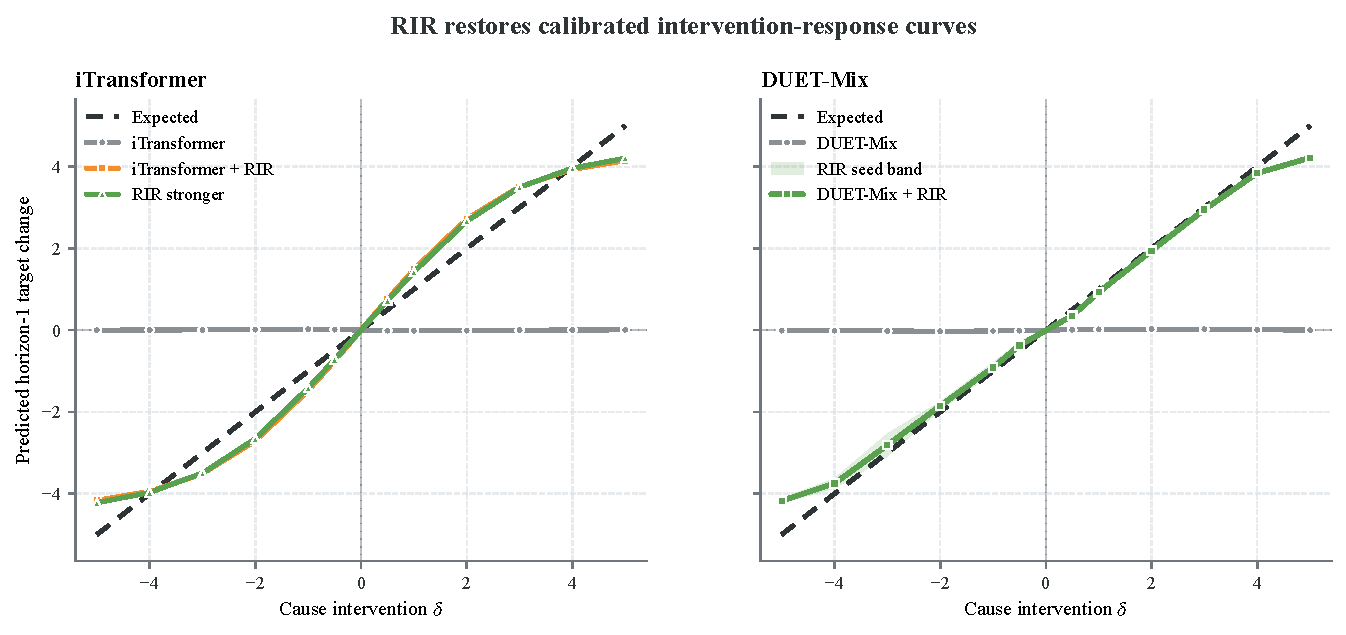
\includegraphics[width=\linewidth]{figures/response_curves_itransformer_duet.pdf}
\caption{Delta-response curves for two channel-mixing architectures. The dashed
line is the expected response. MSE-trained models are nearly flat, while RIR tracks
the intervention-response function across positive and negative shifts.}
\label{fig:main_response_curve}
\end{figure}

\subsection{Semi-Synthetic Real Data: Augmented ETTh1}
\label{sec:etth}

The controlled benchmark provides exact causal labels, but it is synthetic. We
therefore construct an augmented ETTh1 diagnostic: retain all original ETTh1
channels, including \texttt{OT}, and append
\begin{equation}
Y^{\mathrm{rir}}_t
=2\cdot\mathrm{HUFL}_{t-1}+s(t)+\epsilon_t ,
\end{equation}
where $\epsilon_t\sim\mathcal{N}(0,0.05^2)$ and
$s(t)=2[\sin(2\pi h/24)+0.5\cos(2\pi h/24)+0.5\sin(2\pi d/365.25)]$ for hour
$h$ and day-of-year $d$. RIR is applied only to the appended target. Thus raw
\texttt{OT} accuracy is a side-effect diagnostic rather than causal evidence.
Table~\ref{tab:main_etth} shows that RIR recovers the response curve of the
semi-synthetic target without degrading raw \texttt{OT} MSE/MAE.
Appendix~\ref{app:etth2} repeats the same augmented diagnostic on ETTh2 and finds
the same response collapse and repair, with modest dataset-dependent side effects
on raw \texttt{OT}.

This experiment should be interpreted as a side-effect diagnostic rather than as a
claim that raw ETTh1 contains observable causal intervention labels. The appended
target gives us a known response while the original channels preserve realistic
seasonality, scaling, correlations, and timestamp structure. Because \texttt{OT} is
trained and evaluated normally but never receives a response label, its MSE/MAE
tests whether adding response supervision for one channel causes collateral damage
to an ordinary benchmark target. The result suggests that response alignment can be
added locally: it improves the channel for which response knowledge is available
without necessarily degrading unrelated channels optimized under standard
forecasting loss.

\begin{table}[t]
\centering
\caption{Augmented ETTh1 side-effect diagnostic at prediction length 96, reported
as mean $\pm$ standard deviation over three seeds.}
\label{tab:main_etth}
\resizebox{\linewidth}{!}{
\begin{tabular}{lrrrrrr}
\toprule
Variant & All MSE & Raw OT MSE & Raw OT MAE & Semi MSE & Curve slope & Curve IRE \\
\midrule
Baseline & $0.4267{\pm}0.0022$ & $0.0559{\pm}0.0002$ & $0.1828{\pm}0.0004$ & $0.7144{\pm}0.0039$ & $0.0226{\pm}0.0023$ & $2.4149{\pm}0.0056$ \\
+ RIR & $0.4265{\pm}0.0043$ & $0.0557{\pm}0.0005$ & $0.1817{\pm}0.0007$ & $0.7078{\pm}0.0083$ & $0.9292{\pm}0.0121$ & $0.3317{\pm}0.0057$ \\
\bottomrule
\end{tabular}
}
\end{table}

\section{Discussion and Conclusion}
\label{sec:limitations}

Our cleanest evidence uses a linear one-lag synthetic mechanism. This choice makes
the horizon-1 counterfactual response unambiguous, but it does not by itself prove
the same magnitude of blindness for nonlinear, multi-lag, or confounded mechanisms.
The augmented ETT diagnostics improve external validity but remain semi-synthetic;
raw Traffic, Electricity, or ETT benchmarks would test observational accuracy
rather than causal response unless augmented with known response labels. Some core
tables still use single-seed diagnostics or historical checkpoints, while DUET-Mix
and the augmented ETT diagnostics are already evaluated over three seeds. A final
submission should continue
with unified multi-seed reruns and a supplementary reproducibility package.
Finally, RIR assumes known driver-response labels; it is not a general causal
discovery method, and misspecified response labels could align a model to an
incorrect domain belief.

The broader implication is evaluative. Current MLTSF leaderboards reward models for
interpolation on observational test windows. That protocol is appropriate when the
deployment distribution is stable and no controllable driver is changed. It is
insufficient, however, for settings where forecasts are used under policy changes,
control actions, physical inputs, or upstream interventions. In those settings, a
forecasting benchmark should include at least a small number of response-aware unit
tests: known driver interventions, negative-control distractor interventions, and
local response slopes. Such tests do not require solving general causality, but they
prevent a model from looking reliable solely because it follows target-history
autocorrelation.

We identify causal blindness as a hidden failure mode of multivariate time-series
forecasting: low MSE/MAE can coexist with near-zero response to the true driver.
Across representative architectures, including DUET-Mix, the learned functions are
often locally aligned with target-history shortcuts rather than the causal input.
Intervention-aware diagnostics expose this gap, and RIR shows that known response
labels can steer existing forecasters toward the right response without necessarily
damaging ordinary benchmark accuracy.

\iffalse

\section{Related Work}

\paragraph{Multivariate time-series forecasting.}
Modern MLTSF research has explored transformer-based sequence models
\citep{zhou2021informer,wu2021autoformer,zhou2022fedformer}, channel-independent
patch models \citep{nie2023patchtst}, simple linear baselines
\citep{zeng2023transformers}, inverted transformer designs \citep{liu2024itransformer},
cross-dimensional attention \citep{zhang2023crossformer}, multiscale mixing
\citep{wang2024timemixer}, and dual temporal-channel clustering \citep{qiu2025duet}.
These works primarily optimize and report observational
forecasting metrics. Our work is orthogonal: we do not propose another forecasting
backbone, but examine whether existing backbones exhibit correct counterfactual
response under known interventions.

\paragraph{Channel dependence and channel independence.}
A major design question in MLTSF is whether to model channels independently or mix
information across variables. Channel-independent models often perform strongly by
reducing overfitting and exploiting robust univariate temporal patterns. Channel-mixing
models aim to capture cross-variable interactions. Our findings complicate this
dichotomy. Channel-independent models can be structurally unable to use a causal
driver for another target channel, while channel-mixing models may respond to
non-causal channels or still rely predominantly on target self-history. Therefore,
cross-channel mixing is not equivalent to correct causal dependency learning.

\paragraph{Distribution shift and normalization.}
Forecasting models are often evaluated under non-stationarity and distribution shift,
and normalization methods such as reversible instance normalization have been proposed
to improve robustness \citep{kim2022revin}. Our setting differs from standard shift
evaluation: we intervene on known drivers and ask whether the model response matches
the ground-truth mechanism. This highlights a failure that can be hidden by MSE under
the observational distribution.

\paragraph{Shortcut learning and invariance.}
Shortcut learning studies how models exploit predictive but non-causal features when
such features reduce training loss \citep{geirhos2020shortcut}. Related ideas appear
in invariant and causal representation learning, where the goal is to learn predictors
that remain valid under changes in environments or mechanisms
\citep{arjovsky2019invariant,scholkopf2021toward}. Our contribution is narrower and
operational for MLTSF: rather than discovering invariant features from multiple
environments, we test whether a trained forecaster has the correct numerical response
to a known driver intervention. This makes the failure directly measurable with
response slopes and interventional response errors.

\paragraph{Causality and counterfactual forecasting.}
Classical causal reasoning emphasizes interventions and counterfactual responses
\citep{granger1969investigating,pearl2009causality,peters2017elements}. Most MLTSF
benchmarks, however, do not provide intervention labels or causal graphs. We do not
attempt general causal discovery. Instead, we construct forecasting tasks where the
intervention effect is analytically known, allowing us to isolate whether forecasters
learn the response function implied by a known mechanism.

Recent work has begun to connect forecasting more directly with causal evaluation
and counterfactual reasoning. \citet{crasson2024training} train and evaluate causal
forecasting models using orthogonal learning and regression discontinuity designs,
while \citet{yan2023self} generate counterfactual explanations for time-series
predictions. Concurrent contextual forecasting work also explores causal inductive
biases for selecting relevant external signals \citep{yang2025learning}. Our focus
is complementary: rather than estimating treatment effects from observational
settings or generating explanations, we audit whether standard MLTSF forecasters
have the correct numerical response to known driver interventions and provide a
lightweight response regularizer when such labels are available.

\section{Problem Setup}

Let $X_{1:T} \in \mathbb{R}^{T \times N}$ denote a multivariate history window and
$Z_{T+1:T+H} \in \mathbb{R}^{H \times N}$ denote the full multivariate future
window. A forecaster
$f_\theta$ maps
\begin{equation}
\hat{Z}_{T+1:T+H} = f_\theta(X_{1:T}).
\end{equation}
Standard evaluation reports an observational error such as
\begin{equation}
\mathcal{L}_{\mathrm{obs}} =
\frac{1}{HN}\left\|\hat{Z}_{T+1:T+H} - Z_{T+1:T+H}\right\|_F^2.
\end{equation}

We focus on the response of a target channel $y$ to an intervention on a cause
channel $c$. Let $X^a$ be the input obtained by applying intervention $a$ to the
history of $c$. The model's horizon-$h$ predicted response on the target channel is
\begin{equation}
\Delta \hat{y}_{h}(a) = f_\theta(X^a)_{h,y} - f_\theta(X)_{h,y}.
\end{equation}
When the data-generating mechanism specifies a counterfactual future $Z^a$, the
corresponding true target response is
\begin{equation}
\Delta y_{h}(a) = Z^a_{h,y} - Z_{h,y}.
\end{equation}
This paper uses exact counterfactual labels only for $h=1$; multi-step
counterfactual responses require specifying future driver trajectories or full
structural equations for all relevant variables. A model is causally responsive if
$\Delta \hat{y}_{1}(a)$ matches $\Delta y_{1}(a)$ in direction and magnitude for
interventions on true drivers, while remaining stable under interventions on
non-causal distractors.

\paragraph{Causal blindness.}
We define causal blindness as a mismatch between observational accuracy and
interventional response:
\begin{equation}
\mathcal{L}_{\mathrm{obs}} \ \mathrm{is\ low}
\quad \mathrm{but} \quad
\left|\Delta \hat{y}_{1}(a) - \Delta y_{1}(a)\right| \ \mathrm{is\ high}.
\end{equation}
The most severe form occurs when $\Delta \hat{y}_{1}(a)\approx 0$ despite a large nonzero
ground-truth response.

\section{Controlled Causal Forecasting Benchmark}

\subsection{Data generation}

We construct a synthetic multivariate benchmark with $N=21$ channels:
one cause $C$, one target $Y$, and nineteen distractors $D_1,\ldots,D_{19}$.
The cause is a mixed-frequency sinusoidal process with noise. The target follows
the lagged mechanism
\begin{equation}
Y_t = 2 C_{t-1} + \epsilon_t,
\end{equation}
where $\epsilon_t$ is small Gaussian noise. Distractors are generated as independent
periodic or random-walk processes and have no causal effect on $Y$.

We use a history length of $T=96$ and prediction horizon $H=96$. The dataset has
10,000 time steps, split into 70\% training, 10\% validation, and 20\% test.
All variables are standardized once using training-set statistics. Interventions are
then applied in this standardized input space. The target channel is moved to the
final column after loading, yielding the following channel map:
\begin{equation}
\mathrm{channel}\ 0 = C, \quad
\mathrm{channels}\ 1\ldots 19 = D_1,\ldots,D_{19}, \quad
\mathrm{channel}\ 20 = Y.
\end{equation}

\subsection{Interventions}

We use two kinds of interventions. For broad sensitivity diagnostics, we perturb
entire historical channels in standardized input space:
\begin{align}
\mathrm{cause\ shift:} \quad & C_{1:T}' = C_{1:T} + 5, \\
\mathrm{cause\ zero:} \quad & C_{1:T}' = 0, \\
\mathrm{cause\ flip:} \quad & C_{1:T}' = -C_{1:T}, \\
\mathrm{distractor\ shift:} \quad & D_{1:19,1:T}' = D_{1:19,1:T} + 5, \\
\mathrm{target\ zero:} \quad & Y_{1:T}' = 0.
\end{align}

For counterfactual response evaluation, we use a cleaner last-step intervention
\begin{equation}
C'_T = C_T + \delta,\qquad C'_t=C_t \ \mathrm{for}\ t<T.
\end{equation}
Since $Y_{T+1}=2C_T+\epsilon_{T+1}$, this intervention has a known horizon-1 target
response; this is simply Eq.~\eqref{eq:structural} evaluated at $t=T+1$ and does
not require assumptions about future cause trajectories. We use
$\delta=5$ for the main horizon-1 tables and sweep
$\delta \in \{-5,-4,-3,-2,-1,-0.5,0.5,1,2,3,4,5\}$ for response-curve evaluation.

This last-step intervention also avoids a common ambiguity in perturbation tests:
all-history additive shifts can be partially removed by per-instance normalization
inside some forecasting backbones. In all experiments, dataset-level standardization
uses only training statistics, while model-internal normalization layers are left as
implemented by each backbone unless explicitly stated. Our horizon-1 response label
is defined after dataset standardization and before model-internal transformations.

Because variables are standardized, the expected standardized horizon-1 response is
\begin{equation}
\Delta Y^{\mathrm{std}}_{T+1}
= 2 \frac{\sigma_C}{\sigma_Y} \Delta C^{\mathrm{std}}_T.
\label{eq:scaled_response}
\end{equation}
In our benchmark, $2\sigma_C/\sigma_Y = 1.000076888$, so a standardized cause shift
of $+5$ implies an expected horizon-1 target change of approximately $5.000384$.

\section{Intervention-Aware Metrics}

\paragraph{Mean prediction difference.}
For intervention $a$, we define the target mean prediction difference as
\begin{equation}
\mpd(a) =
\mathbb{E}\left[
\left| f_\theta(X^a)_{1,Y} - f_\theta(X)_{1,Y} \right|
\right],
\end{equation}
where $f_\theta(\cdot)_{1,Y}$ denotes the horizon-1 prediction for the target channel.
We also report the same quantity over all horizons in sensitivity experiments.

\paragraph{Horizon-1 interventional response error.}
When the counterfactual label is known, we define
\begin{equation}
\ire_{H1}(a) =
\mathbb{E}\left[
\left|
\left(f_\theta(X^a)_{1,Y} - f_\theta(X)_{1,Y}\right)
-
\left(Z^a_{1,Y} - Z_{1,Y}\right)
\right|
\right].
\end{equation}

\paragraph{Response slope.}
For interventions that induce nonzero true responses, we compute the slope of predicted
response against true response:
\begin{equation}
\mathrm{slope}
=
\frac{\sum_i \Delta \hat{y}_{1,i} \Delta y_{1,i}}{\sum_i (\Delta y_{1,i})^2}.
\end{equation}
An ideal model has slope near 1. A slope near 0 indicates causal blindness.

\paragraph{Sign accuracy.}
We also report the fraction of windows for which the predicted response has the same
sign as the true response. This captures directional correctness even when magnitude
is miscalibrated.

\paragraph{Response ratio.}
For delta-response curves, we additionally report the mean response ratio
$\mathbb{E}_\delta[\bar{\Delta\hat{y}}_1(\delta)/\Delta y_1(\delta)]$ over
nonzero intervention magnitudes. This is a signed calibration summary; values near
one indicate well-calibrated response magnitude.

\section{Experiments}

\subsection{Models}

We evaluate five representative forecasting architectures:
\begin{itemize}[leftmargin=*]
    \item DLinear, a simple linear decomposition baseline;
    \item PatchTST, a channel-independent patch transformer;
    \item iTransformer, an inverted transformer with variable tokens;
    \item Crossformer, a cross-dimensional transformer;
    \item TimeMixer, a modern multiscale mixing model.
\end{itemize}

All models are trained or evaluated in the same Time-Series-Library codebase with
history length 96 and horizon length 96. PatchTST, iTransformer, and Crossformer use
historical checkpoints recovered from the original experiment directory. DLinear and
TimeMixer are trained in the current reproduction run. Unless otherwise specified,
results are single-seed diagnostics; we return to this limitation in
Section~\ref{sec:limitations}.

We additionally evaluate DUET, a recent dual-clustering multivariate forecasting
model, using an independent clean script that calls the repository's original
\texttt{forward\_()} implementation. This is necessary because the inspected server
copy contained an earlier debug modification in \texttt{forward()} for intervention
visualization.

\subsection{Sensitivity results}

Table~\ref{tab:sensitivity} reports target-channel observational error and prediction
sensitivity under cause, distractor, and target-history interventions. The pattern is
consistent: cause interventions induce near-zero target response, while target-history
interventions strongly change the forecast.

\begin{table}[t]
\centering
\caption{Sensitivity evaluation on the controlled causal benchmark. Lower MSE/MAE
does not imply stronger response to the true cause. TimeMixer obtains the lowest
target MSE but has zero response to a cause shift.}
\label{tab:sensitivity}
\resizebox{\linewidth}{!}{
\begin{tabular}{lrrrrr}
\toprule
Model & Target MSE & Target MAE & Cause MPD & Distractor MPD & Target-zero MPD \\
\midrule
DLinear      & 0.545448 & 0.622045 & 0.000000 & 0.000000 & 0.562089 \\
PatchTST     & 0.296033 & 0.427234 & 0.000000 & 0.000000 & 0.730165 \\
iTransformer & 0.060812 & 0.190868 & 0.000002 & 0.000006 & 0.840644 \\
Crossformer  & 0.015730 & 0.099358 & 0.003551 & 0.034936 & 0.878338 \\
TimeMixer    & 0.010938 & 0.083087 & 0.000000 & 0.000000 & 0.857566 \\
\bottomrule
\end{tabular}
}
\end{table}

The TimeMixer result is especially revealing. It has the lowest observational target
MSE among the tested models, yet its response to the true cause shift is exactly zero
under this evaluation. Because the all-history shift in Table~\ref{tab:sensitivity}
can be attenuated by per-instance normalization, we use it only as a broad
sensitivity diagnostic. The cleaner causal evidence comes from the last-step
interventions in Tables~\ref{tab:duet}--\ref{tab:small_delta}, which alter the
local sequence shape and have analytic horizon-1 responses. Crossformer is also
instructive: it responds more to distractor shifts than to the true cause shift,
suggesting that cross-channel mixing does not guarantee correct causal dependency
learning.

DUET strengthens this conclusion. Table~\ref{tab:duet} reports three DUET variants:
a channel-independent setting trained with MSE, a channel-mixing setting trained with
MSE, and a channel-independent setting trained with MAE to match the common DUET
benchmark protocol. All three obtain low observational error but near-zero
horizon-1 response to the true cause.

\begin{table}[t]
\centering
\caption{Additional DUET evaluation. The expected standardized horizon-1 response
under a last-cause intervention of $+5$ is $5.000384$. DUET obtains low target MSE
but still predicts near-zero causal response.}
\label{tab:duet}
\begin{tabular}{lrrrrrr}
\toprule
Variant & Loss & Target MSE & Target MAE & Pred. $|\Delta|$ & H1 IRE & Slope \\
\midrule
DUET-CI  & MSE & 0.018961 & 0.111400 & 0.029323 & 4.998435 & 0.000390 \\
DUET-Mix & MSE & 0.024529 & 0.126233 & 0.052558 & 4.998288 & 0.000419 \\
DUET-CI  & MAE & 0.027745 & 0.134924 & 0.040672 & 4.974961 & 0.005084 \\
\bottomrule
\end{tabular}
\end{table}

\subsection{Counterfactual horizon-1 response}

Table~\ref{tab:h1} evaluates the response to a cause shift of $+5$. Under the known
mechanism, the expected standardized horizon-1 target change is $5.000384$. All five
models produce responses near zero. The resulting response slopes are also near zero.

\begin{table}[t]
\centering
\caption{Counterfactual horizon-1 response to a standardized cause shift of $+5$.
The expected target response is analytically known from Eq.~\eqref{eq:scaled_response}.
All models produce near-zero response, despite large target-history sensitivity.}
\label{tab:h1}
\begin{tabular}{lrrrrr}
\toprule
Model & Expected & Pred. $|\Delta|$ & H1 IRE & Response Slope & Target-zero MPD \\
\midrule
DLinear      & 5.000384 & 0.000000 & 5.000384 & 0.000000 & 0.648138 \\
PatchTST     & 5.000384 & 0.000000 & 5.000384 & 0.000000 & 0.798587 \\
iTransformer & 5.000384 & 0.032361 & 4.993866 & 0.001304 & 0.869898 \\
Crossformer  & 5.000384 & 0.000660 & 4.999750 & 0.000127 & 0.884160 \\
TimeMixer    & 5.000384 & 0.000000 & 5.000384 & 0.000000 & 0.837711 \\
\bottomrule
\end{tabular}
\end{table}

These results support a stronger conclusion than ordinary perturbation sensitivity:
even when the correct counterfactual response is known analytically, standard
forecasters can fail to produce it. Moreover, these models are not simply invariant
to all changes. They strongly respond to target-history perturbations, which have no
counterfactual effect under the structural equation when the cause is unchanged.

\subsection{Linear sanity baselines and small interventions}

To check that the evaluation pipeline itself can recover the correct response, we
fit elementary linear horizon-1 baselines under the same global standardization and
test split. Table~\ref{tab:linear_sanity} shows that an autoregressive target-only
baseline obtains reasonable observational error but has zero response to the cause,
whereas ARX and VARX baselines that explicitly use the last cause value recover a
response slope near one. This confirms that the near-zero response of deep
forecasters is not caused by the standardization or intervention pipeline.

\begin{table}[t]
\centering
\caption{Linear sanity baselines under the same preprocessing and horizon-1
evaluation. ``Small'' uses $\delta \in \{\pm0.1,\pm0.25,\pm0.5,\pm1\}$, while
``Full'' uses the wider sweep in Table~\ref{tab:response_curve}. A correctly
specified ARX baseline recovers the expected response.}
\label{tab:linear_sanity}
\begin{tabular}{lrrrrr}
\toprule
Model & H1 MSE & H1 MAE & Cause coef. & Small slope & Full slope \\
\midrule
AR($Y_T$) & 0.0183 & 0.1096 & 0.0000 & 0.0000 & 0.0000 \\
ARX($C_T$) & 0.0010 & 0.0251 & 0.9996 & 0.9995 & 0.9995 \\
ARX($C_T,Y_T$) & 0.0010 & 0.0251 & 1.0037 & 1.0036 & 1.0036 \\
VARX($X_T$) & 0.0010 & 0.0253 & 1.0040 & 1.0039 & 1.0039 \\
\bottomrule
\end{tabular}
\end{table}

We also test whether causal blindness is only an artifact of the large $\delta=5$
intervention. Table~\ref{tab:small_delta} evaluates a smaller local sweep
$\delta \in \{\pm0.1,\pm0.25,\pm0.5,\pm1\}$. The MSE-trained deep forecasters still
have near-zero slopes, while the ARX baseline remains calibrated. RIR restores
sign-correct local responsiveness, although FT01 is over-responsive in this small
range; we view this as a calibration trade-off rather than as a failure of the
diagnostic.

\begin{table}[t]
\centering
\caption{Small-delta response evaluation. The flat response is already visible in
the local perturbation regime, so it is not only a large-OOD-shift artifact.}
\label{tab:small_delta}
\begin{tabular}{lrrr}
\toprule
Model & Small-delta slope & Mean IRE & Mean ratio \\
\midrule
ARX($C_T$) & 0.9995 & 0.0002 & 0.9995 \\
iTransformer & -0.0220 & 0.4737 & -0.0273 \\
iTransformer + RIR FT01 & 1.4769 & 0.2304 & 1.4955 \\
PatchTST & 0.0000 & 0.4625 & 0.0000 \\
Crossformer & 0.0000 & 0.4625 & 0.0000 \\
TimeMixer & 0.0000 & 0.4625 & 0.0000 \\
\bottomrule
\end{tabular}
\end{table}

\subsection{Failure taxonomy}

Our results suggest three failure patterns:
\begin{itemize}[leftmargin=*]
    \item \textbf{Structural blindness.} Strict channel-independent predictors such
    as DLinear and PatchTST can be structurally unable to transfer information from
    the cause channel to the target channel, yielding exactly zero target response
    under MSE training.
    \item \textbf{Lazy causal learning.} Channel-mixing models such as iTransformer
    can have access to all variables but still learn a target-history shortcut, leading
    to weak or negligible cause response.
    \item \textbf{Spurious cross-channel sensitivity.} Cross-dimensional models such
    as Crossformer may respond to non-causal distractors more than to the true cause,
    indicating that cross-channel interaction is not necessarily causal interaction.
\end{itemize}

\section{Why Does Causal Blindness Emerge?}

Causal blindness can arise because observational prediction error does not identify
the model's response function. Consider a target generated by
$Y_{T+1}=g(C_T)+\epsilon$, where $C_T$ is the true driver. If the target history
$S=X_{1:T,Y}$ is highly predictive under the observational distribution, a model
$f_\theta(X)=h_\theta(S)$ can obtain low MSE whenever
$\mathbb{E}(Y_{T+1}-h_\theta(S))^2$ is small. However, this predictor has
$\partial f_\theta/\partial C_T \approx 0$ and therefore fails under an intervention
on the driver. In other words, observational MSE constrains the value of the
prediction on observed samples, but it does not constrain the local derivative or
finite response with respect to the causal input. This creates an optimization path
where target-history shortcuts are sufficient for accuracy but insufficient for
interventional correctness.

A simple formal intuition makes this gap explicit. Suppose
$C_T=q(S)+\nu$ under the observational distribution, with
$\mathbb{E}\nu^2\leq \eta^2$, and suppose $g$ is $L$-Lipschitz. Then the
shortcut predictor $h(S)=g(q(S))$ satisfies
\begin{equation}
\mathbb{E}\left(Y_{T+1}-h(S)\right)^2
\leq
L^2\eta^2 + \mathbb{E}\epsilon^2,
\end{equation}
when the structural noise is mean-zero and independent of $\nu$; a looser constant
factor bound also holds without this independence. Thus it can be observationally
accurate whenever the target history predicts the driver well on the training
manifold. Under an intervention
$C_T \leftarrow C_T+\delta$, however, this same predictor has zero response, while
the structural response is $g(C_T+\delta)-g(C_T)$. For the linear mechanism used in
our benchmark, this missed response is proportional to $|\delta|$ even if
observational MSE is small. Thus the failure is not paradoxical: the training loss
can select a function that agrees with the data manifold but has the wrong
off-manifold or interventional response.

This perspective also clarifies the role of architecture. Channel-independent models
can be blind because the target prediction path does not use other channels. In
channel-mixing models, the cause is accessible, but access is not alignment: the
training loss may still prefer target-history features if they provide a cheaper
route to low observational error. We test this explanation by measuring functional
input sensitivity. For a small standardized finite-difference step $\tau=0.05$, we compute
\begin{equation}
S(a)=
\mathbb{E}\left[
\left|
\frac{f_\theta(X+\tau a)_{1,Y}-f_\theta(X-\tau a)_{1,Y}}{2\tau}
\right|
\right],
\end{equation}
where $a$ perturbs either the last cause value or the last target-history value.
Table~\ref{tab:functional_sensitivity} shows that the MSE-only iTransformer is much
less sensitive to the last cause value than to the last target value
($0.032$ vs. $0.239$). MSE-only fine-tuning does not remove this imbalance. In
contrast, RIR raises cause-last sensitivity above target-last sensitivity, matching
the intended response behavior. PatchTST and TimeMixer have zero cause-last
sensitivity, consistent with their zero interventional response. These results
support the interpretation that causal blindness is not merely a metric artifact:
the learned functions are locally insensitive to the true driver.

\begin{table}[t]
\centering
\caption{Functional input sensitivity of the horizon-1 target prediction, measured
by central differences with $\tau=0.05$ over 32 test batches. MSE-only models are
far more sensitive to target history than to the true last-step cause. RIR changes
the local response geometry of iTransformer.}
\label{tab:functional_sensitivity}
\resizebox{\linewidth}{!}{
\begin{tabular}{lrrrr}
\toprule
Model & Cause-last sens. & Target-last sens. & Cause/Target & Cause-history sens. \\
\midrule
iTransformer & 0.0318 & 0.2385 & 0.133 & 0.000004 \\
iTransformer MSE fine-tune & 0.0396 & 0.2015 & 0.196 & 0.000007 \\
iTransformer + RIR FT01 & 1.5075 & 1.3417 & 1.124 & 0.000020 \\
iTransformer + RIR FT03 & 1.4344 & 1.4019 & 1.023 & 0.000018 \\
PatchTST & 0.0000 & 0.5362 & 0.000 & 0.000000 \\
Crossformer & 0.0001 & 0.0483 & 0.002 & 0.001234 \\
TimeMixer & 0.0000 & 0.1752 & 0.000 & 0.000000 \\
\bottomrule
\end{tabular}
}
\end{table}

\section{\rir{}}

The goal of this paper is not to solve general causal discovery. In many settings,
domain knowledge or benchmark construction can identify a driver and its expected
intervention response. In such cases, we can regularize the forecast response directly.

During RIR training, we sample a signed intervention magnitude
$\delta_i=s_i m_i$, where $s_i\in\{-1,1\}$ is uniform and
$m_i\sim\mathrm{Uniform}(\rho\Delta_{\max},\Delta_{\max})$. For the iTransformer
synthetic experiments we use $\Delta_{\max}=5$ and $\rho=0.5$; DUET and ETTh1
augmented runs use $\rho=0.1$. The causal intervention changes only the last
historical driver value, $C_T\leftarrow C_T+\delta_i$, and the expected standardized
horizon-1 target response is $\Delta y_i^\star=(2\sigma_C/\sigma_Y)\delta_i$.
We define the response loss on the horizon-1 target slice:
\begin{equation}
\mathcal{L}_{\mathrm{resp}}
=
\frac{1}{B}\sum_{i=1}^{B}
\left[
f_\theta(X_i^{\mathrm{cf}})_{1,Y}
-
f_\theta(X_i)_{1,Y}
-
\Delta y_i^\star
\right]^2.
\end{equation}
For distractor interventions, we add an independently sampled signed magnitude to
the last historical values of the distractor channels and set the expected target
response to zero:
\begin{equation}
\mathcal{L}_{\mathrm{dist}}
=
\frac{1}{B}\sum_{i=1}^{B}
\left[
f_\theta(X_i^{\mathrm{dist}})_{1,Y}
-
f_\theta(X_i)_{1,Y}
\right]^2.
\end{equation}
The total training objective is
\begin{equation}
\mathcal{L}
=
\mathcal{L}_{\mathrm{pred}}
+
\lambda_1 \mathcal{L}_{\mathrm{resp}}
+
\lambda_2 \mathcal{L}_{\mathrm{dist}}.
\label{eq:rir}
\end{equation}

This objective, which we call \rir{}, encourages the model to respond to true causal
drivers while remaining stable under distractor perturbations. It introduces no new
parameters but requires three forward passes per training step: original, causal
intervention, and distractor intervention. We instantiate this objective on
iTransformer in three settings. FT01 and FT03 initialize
from the MSE-only checkpoint and fine-tune with
$(\lambda_1,\lambda_2)=(0.1,0.01)$ and $(0.3,0.03)$, respectively; the scratch
variant trains with RIR from random initialization using
$(\lambda_1,\lambda_2)=(1.0,0.1)$. Table~\ref{tab:rir} shows that
RIR converts the baseline from an almost non-responsive predictor into one that
tracks the known horizon-1 intervention response. The fine-tuned variants retain far
more observational accuracy than the scratch variant, suggesting a practical
accuracy--response trade-off rather than an all-or-nothing repair.

\begin{table}[t]
\centering
\caption{RIR results on iTransformer. The expected horizon-1 target
response under a standardized last-cause intervention of $+5$ is $5.000$. FT01 and
FT03 are initialized from the MSE-only checkpoint.}
\label{tab:rir}
\begin{tabular}{lrrrrr}
\toprule
Model & Target MSE & Target MAE & Pred. $\Delta$ & H1 IRE & Slope \\
\midrule
iTransformer & 0.0608 & 0.1909 & 0.032 & 4.994 & 0.001 \\
+ RIR FT01 & 0.1054 & 0.2553 & 4.149 & 0.871 & 0.830 \\
+ RIR FT03 & 0.1465 & 0.3020 & 4.205 & 0.816 & 0.841 \\
+ RIR scratch & 0.5308 & 0.5910 & 4.794 & 0.243 & 0.959 \\
\bottomrule
\end{tabular}
\end{table}

We further run a targeted ablation to separate causal response learning from extra
fine-tuning. Table~\ref{tab:rir_ablation} shows that MSE-only fine-tuning leaves the
model nearly causally blind, while response-only RIR learns the desired cause response
but also becomes highly reactive to last-step distractor interventions. Adding the
distractor stability term reduces this false response by almost an order of magnitude,
although it does not yet return to the baseline level. This suggests that both terms
are useful: $\mathcal{L}_{\mathrm{resp}}$ teaches the model to respond to the known
driver, and $\mathcal{L}_{\mathrm{dist}}$ prevents response learning from becoming
indiscriminate reactivity.

\begin{table}[t]
\centering
\caption{RIR ablation on iTransformer. ``Last-dist.'' reports the absolute
horizon-1 target change under a last-step distractor intervention, whose expected
effect is zero.}
\label{tab:rir_ablation}
\begin{tabular}{lrrrrr}
\toprule
Model & Target MSE & Cause response & H1 IRE & Slope & Last-dist. false resp. \\
\midrule
iTransformer & 0.0608 & 0.032 & 4.994 & 0.001 & 0.200 \\
MSE fine-tune & 0.0826 & 0.062 & 4.987 & 0.003 & 0.262 \\
+ $\mathcal{L}_{\mathrm{resp}}$ & 0.1095 & 4.277 & 0.755 & 0.855 & 5.929 \\
+ $\mathcal{L}_{\mathrm{resp}}+\mathcal{L}_{\mathrm{dist}}$ & 0.1054 & 4.149 & 0.871 & 0.830 & 0.672 \\
\bottomrule
\end{tabular}
\end{table}

Finally, we test whether the repair holds beyond the single $+5$ intervention used
in Table~\ref{tab:rir}. We sweep positive and negative intervention magnitudes
$\delta \in \{-5,-4,-3,-2,-1,-0.5,0.5,1,2,3,4,5\}$ and compare the predicted
horizon-1 response against the analytically expected response
$(2\sigma_C/\sigma_Y)\delta$. Table~\ref{tab:response_curve} and
Figure~\ref{fig:response_curve} show that the MSE-only iTransformer collapses to an
almost flat response curve, while RIR recovers an approximately linear,
sign-correct response over the intervention range. MSE-only fine-tuning does not
repair the curve, indicating that the effect comes from response supervision rather
than additional optimization alone.

\begin{table}[t]
\centering
\caption{Delta-response curve evaluation on iTransformer variants. Slope and
correlation are computed from mean predicted response across intervention magnitudes.
The baseline and MSE-only fine-tuning remain nearly flat, while response supervision
recovers the causal response curve.}
\label{tab:response_curve}
\begin{tabular}{lrrrr}
\toprule
Model & Curve slope & Curve corr. & Mean IRE & Mean ratio \\
\midrule
iTransformer & -0.0008 & -0.2276 & 2.5913 & -0.0090 \\
MSE fine-tune & -0.0001 & -0.0126 & 2.5906 & -0.0103 \\
+ $\mathcal{L}_{\mathrm{resp}}$ & 0.9969 & 0.9865 & 0.5112 & 1.2178 \\
+ $\mathcal{L}_{\mathrm{resp}}+\mathcal{L}_{\mathrm{dist}}$ & 0.9836 & 0.9839 & 0.5447 & 1.2216 \\
+ RIR FT03 & 0.9867 & 0.9862 & 0.5096 & 1.1983 \\
\bottomrule
\end{tabular}
\end{table}

\begin{figure}[t]
\centering
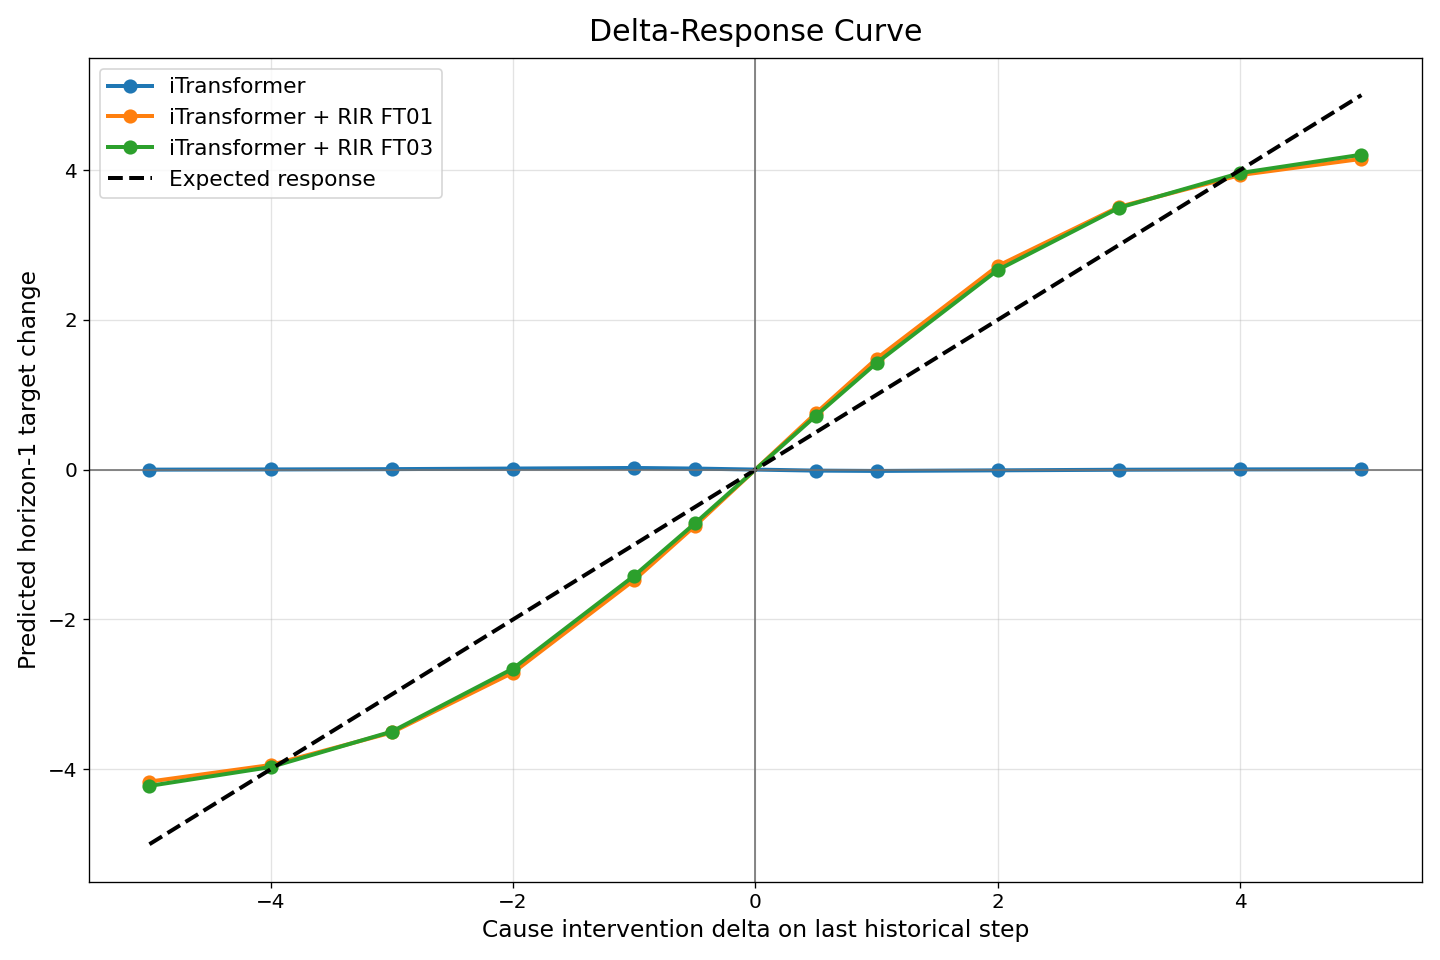
\includegraphics[width=0.78\linewidth]{../results/delta_response_itransformer_crr_curve_20260503/delta_response_curve.png}
\caption{Delta-response curves for iTransformer and RIR variants. The dashed
line is the expected response. The MSE-only model stays near zero across positive
and negative cause interventions, whereas RIR tracks the expected response
function.}
\label{fig:response_curve}
\end{figure}

To test whether response regularization is specific to iTransformer, we also apply it
to DUET-Mix, the channel-mixing variant of DUET. Table~\ref{tab:duet_crr} and
Figure~\ref{fig:duet_response_curve} show that DUET-Mix can also be steered toward
the correct response function. Compared with the DUET-Mix baseline, the repaired
model raises the predicted $+5$ response from $0.054\pm0.002$ to
$4.259\pm0.086$ across three seeds, while keeping target MAE comparable to the
baseline. The DUET-Mix baseline has a nearly flat delta-response curve in the
available curve run, whereas the repaired model has curve slope
$0.909\pm0.009$ and low curve IRE across three seeds. Its last-step distractor false
response remains small. This suggests that channel interaction alone does not
guarantee causal response, but intervention-aware supervision can make a
channel-interaction model responsive for the right reason.

\begin{table}[t]
\centering
\caption{DUET-Mix repair with randomized response regularization, reported as
mean $\pm$ standard deviation across three seeds. The baseline has low
observational error but near-zero cause response. RIR recovers most of the expected
H1 effect and substantially reduces target-history sensitivity. Curve statistics for
the baseline are available for one seed; RIR curve statistics are computed over
three seeds.}
\label{tab:duet_crr}
\resizebox{\linewidth}{!}{
\begin{tabular}{lrrrrrrrr}
\toprule
Model & $n$ & Target MSE & Target MAE & Cause resp. & H1 IRE & H1 slope & Target-zero & Curve slope \\
\midrule
DUET-Mix & 3 & $0.0237{\pm}0.0017$ & $0.1245{\pm}0.0043$ & $0.054{\pm}0.002$ & $4.982{\pm}0.017$ & $0.004{\pm}0.003$ & $0.789{\pm}0.011$ & $0.004$ \\
DUET-Mix + RIR & 3 & $0.0308{\pm}0.0066$ & $0.1224{\pm}0.0084$ & $4.259{\pm}0.086$ & $0.744{\pm}0.091$ & $0.852{\pm}0.017$ & $0.342{\pm}0.016$ & $0.909{\pm}0.009$ \\
DUET-CI + RIR & 1 & $0.0273$ & $0.1149$ & $4.506$ & $0.497$ & $0.901$ & $0.333$ & $0.929$ \\
\bottomrule
\end{tabular}
}
\end{table}

The DUET-CI + RIR row should be interpreted as an implementation-specific diagnostic
rather than as evidence that a strictly channel-independent function can use another
channel at inference. The DUET implementation contains shared training components and
auxiliary mechanisms, so response supervision can still alter the learned predictor.
We therefore use DLinear and PatchTST as the stricter channel-independent negative
controls.

\begin{figure}[t]
\centering
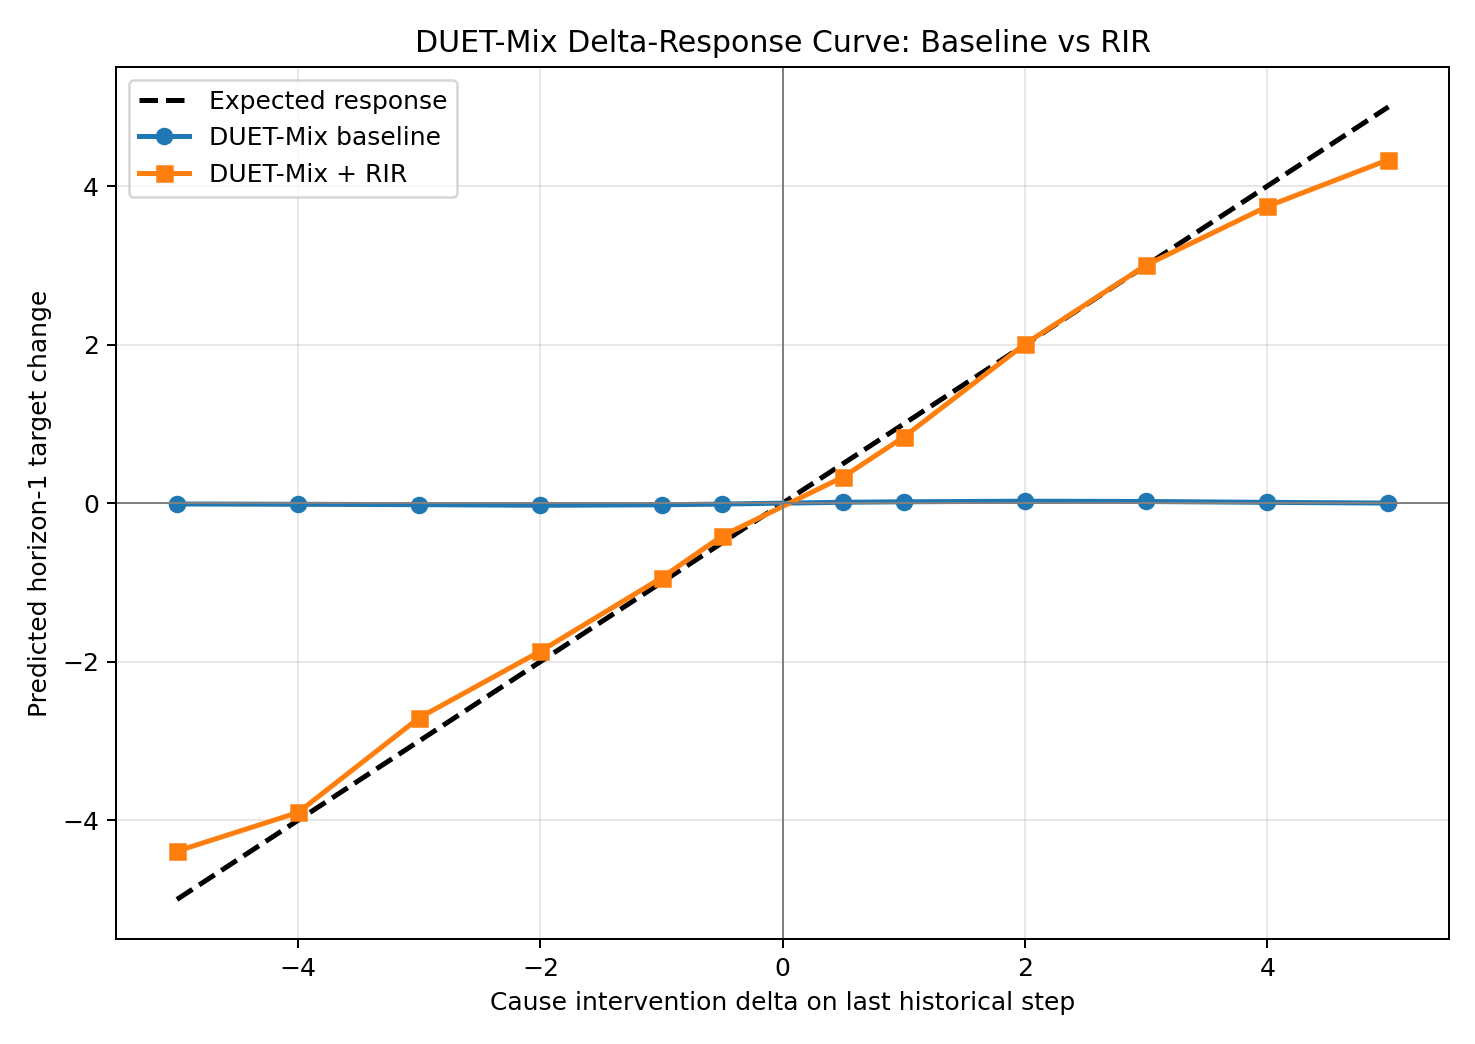
\includegraphics[width=0.78\linewidth]{../results/duet_crr_20260503/duet_baseline_vs_rir_curve.png}
\caption{DUET-Mix delta-response curves. The baseline obtains low observational
error but its response curve collapses near zero. With randomized response
regularization, DUET-Mix tracks the analytically expected intervention-response
function across positive and negative cause shifts.}
\label{fig:duet_response_curve}
\end{figure}

\section{Augmented ETTh1 Side-Effect Diagnostic}

The controlled benchmark provides clean causal evidence, but it is synthetic. To
test whether the same response-collapse phenomenon appears on real benchmark inputs,
and to examine whether response regularization damages ordinary forecasting accuracy,
we construct an augmented ETTh1 diagnostic. We retain all original ETTh1 variables,
including the raw \texttt{OT} channel, and append a semi-synthetic target:
\begin{equation}
Y^{\mathrm{rir}}_t = 2 \cdot \mathrm{HUFL}_{t-1} + s(t) + \epsilon_t,
\end{equation}
where $\epsilon_t\sim\mathcal{N}(0,0.05^2)$ and
\begin{equation}
s(t)=2\left[
\sin(2\pi\,\mathrm{hour}(t)/24)
+0.5\cos(2\pi\,\mathrm{hour}(t)/24)
+0.5\sin(2\pi\,\mathrm{day}(t)/365.25)
\right].
\end{equation}
This setup preserves the real
covariate distribution and timestamp structure of ETTh1 while retaining an analytic
horizon-1 response from \texttt{HUFL} to the appended target. We train iTransformer to
forecast all channels and apply RIR only to the appended target, using
$(\lambda_1,\lambda_2)=(0.05,0.005)$ for the ETTh1 augmented runs. The original
\texttt{OT} channel is never given a response label, so its MSE/MAE serves as a
side-effect diagnostic rather than as causal evidence. Table~\ref{tab:etth_side_effect}
shows that, across three seeds at prediction length 96, RIR recovers the
semi-synthetic response curve without degrading raw \texttt{OT} forecasting accuracy.
We also include a one-seed prediction-length-192 probe, which shows the same
qualitative pattern.

\begin{table}[t]
\centering
\caption{ETTh1 augmented side-effect diagnostic. The original ETTh1 \texttt{OT}
channel is retained and a semi-synthetic target with known response to \texttt{HUFL}
is appended. RIR improves response correctness of the appended target while raw
\texttt{OT} MSE/MAE does not increase. Results for prediction length 96 are reported
as mean $\pm$ standard deviation over three seeds; prediction length 192 is a
single-seed probe.}
\label{tab:etth_side_effect}
\resizebox{\linewidth}{!}{
\begin{tabular}{llrrrrrr}
\toprule
Pred. len & Variant & All MSE & Raw OT MSE & Raw OT MAE & Semi MSE & Curve slope & Curve IRE \\
\midrule
96 & Baseline & $0.4267{\pm}0.0022$ & $0.0559{\pm}0.0002$ & $0.1828{\pm}0.0004$ & $0.7144{\pm}0.0039$ & $0.0226{\pm}0.0023$ & $2.4149{\pm}0.0056$ \\
96 & + RIR & $0.4265{\pm}0.0043$ & $0.0557{\pm}0.0005$ & $0.1817{\pm}0.0007$ & $0.7078{\pm}0.0083$ & $0.9292{\pm}0.0121$ & $0.3317{\pm}0.0057$ \\
192 & Baseline & $0.4906$ & $0.0728$ & $0.2081$ & $0.8375$ & $0.0147$ & $2.4349$ \\
192 & + RIR & $0.4838$ & $0.0728$ & $0.2071$ & $0.8220$ & $0.9531$ & $0.3082$ \\
\bottomrule
\end{tabular}
}
\end{table}

\section{Discussion and Limitations}
\label{sec:limitations}

Our results show that standard forecasting metrics can hide incorrect causal response.
This does not mean that all forecasting tasks require causal modeling. If the test
distribution remains observational and stable, target-history shortcuts may be useful.
However, in settings involving interventions, policies, domain shifts, or controllable
drivers, response correctness becomes essential.

This draft has several limitations. First, the cleanest evidence comes from a
controlled synthetic benchmark with a strong linear, one-lag mechanism. This design
is intentional: it makes the horizon-1 counterfactual response unambiguous, so a
near-zero response cannot be attributed to causal-label uncertainty. It does not by
itself prove that the same magnitude of blindness holds for nonlinear, multi-lag, or
confounded mechanisms. Second, the augmented ETTh1 experiment improves external
validity, but it remains semi-synthetic because raw ETTh1 does not provide
ground-truth intervention labels. Third, although DUET-Mix and ETTh1 augmented
diagnostics are now evaluated over three seeds, the five-model failure table and
iTransformer repair table still require multi-seed reruns before submission. Fourth,
some models were evaluated from historical checkpoints while others were newly
trained; a final version should rerun all models under unified scripts. Fifth, the
current counterfactual label is horizon-1, because only the first future step is
directly determined by the last historical cause without assuming future cause
trajectories. Extending to multi-horizon counterfactual response requires generating
future cause paths or specifying structural equations for future drivers. Finally,
RIR assumes that the driver and its expected response are known from domain knowledge
or benchmark construction; it is not a general causal discovery method.

The broader impact of this work is primarily diagnostic. Response-aware evaluation
may improve reliability in domains such as energy, traffic, and operations where
forecasts are used under interventions or policy changes. The main risk is
over-trusting response diagnostics or RIR when the assumed driver, sign, or response
magnitude is misspecified. In such cases, the regularizer could align a model to an
incorrect domain belief. We therefore view RIR as appropriate only when intervention
labels come from trusted physical knowledge, controlled simulators, or validated
benchmark construction.

\section{Conclusion}

We identify causal blindness as a hidden failure mode in multivariate time-series
forecasting. Across representative architectures, including a recent DUET baseline,
models that achieve reasonable or even low observational error can produce near-zero response to a true causal driver
whose intervention effect is analytically known. At the same time, the same models
strongly respond to target-history perturbations that should not alter the counterfactual
future under the structural equation. These findings suggest that MSE/MAE leaderboards
are insufficient for evaluating forecasting models in settings where response to drivers
matters. Intervention-aware evaluation and lightweight response regularization provide
a path toward forecasters that are not only accurate, but responsive for the right reasons.

\fi

\clearpage

\bibliographystyle{plainnat}
\bibliography{references}

\appendix

\section{Benchmark, Interventions, and Metrics}
\label{app:benchmark}

\paragraph{Data and channel map.}
The controlled benchmark contains one cause $C$, one target $Y$, and 19
distractors. We use 10,000 time steps, split into 70\% training, 10\% validation,
and 20\% test. The history length and prediction horizon are both 96. Variables are
standardized using training-set statistics and then reordered as
channel 0 = $C$, channels 1--19 = distractors, and channel 20 = $Y$.

\paragraph{All-history sensitivity interventions.}
For broad sensitivity diagnostics, we perturb entire historical channels in
standardized input space:
\begin{align}
\mathrm{cause\ shift:}\quad & C'_{1:T}=C_{1:T}+5, &
\mathrm{cause\ zero:}\quad & C'_{1:T}=0, \\
\mathrm{cause\ flip:}\quad & C'_{1:T}=-C_{1:T}, &
\mathrm{distractor\ shift:}\quad & D'_{1:19,1:T}=D_{1:19,1:T}+5,\\
\mathrm{target\ zero:}\quad & Y'_{1:T}=0 .
\end{align}
All-history additive shifts can be attenuated by per-instance normalization inside
some forecasting backbones, so the main causal evidence in the paper uses last-step
interventions with analytic horizon-1 labels.

\paragraph{Metrics.}
For an intervention $a$, mean prediction difference is
\begin{equation}
\mpd(a)=
\mathbb{E}\left[
\left|f_\theta(X^a)_{1,Y}-f_\theta(X)_{1,Y}\right|
\right].
\end{equation}
When the counterfactual label is known, horizon-1 interventional response error is
\begin{equation}
\ire_{H1}(a)=
\mathbb{E}\left[
\left|
\left(f_\theta(X^a)_{1,Y}-f_\theta(X)_{1,Y}\right)
-
\left(Z^a_{1,Y}-Z_{1,Y}\right)
\right|
\right].
\end{equation}
The signed response slope is
\begin{equation}
\mathrm{slope}
=
\frac{\sum_i \Delta\hat{y}_{1,i}\Delta y_{1,i}}
{\sum_i(\Delta y_{1,i})^2}.
\end{equation}
For response curves, we also report the mean signed response ratio over nonzero
intervention magnitudes.

\section{Additional Causal-Blindness Diagnostics}
\label{app:sanity}

\begin{table}[htbp]
\centering
\caption{All-history sensitivity evaluation. This diagnostic is useful for
identifying target-history reliance, but all-history additive shifts can interact
with model-internal normalization.}
\label{tab:app_sensitivity}
\resizebox{\linewidth}{!}{
\begin{tabular}{lrrrrr}
\toprule
Model & Target MSE & Target MAE & Cause MPD & Distractor MPD & Target-zero MPD \\
\midrule
DLinear      & 0.545448 & 0.622045 & 0.000000 & 0.000000 & 0.562089 \\
PatchTST     & 0.296033 & 0.427234 & 0.000000 & 0.000000 & 0.730165 \\
iTransformer & 0.060812 & 0.190868 & 0.000002 & 0.000006 & 0.840644 \\
Crossformer  & 0.015730 & 0.099358 & 0.003551 & 0.034936 & 0.878338 \\
TimeMixer    & 0.010938 & 0.083087 & 0.000000 & 0.000000 & 0.857566 \\
\bottomrule
\end{tabular}
}
\end{table}

\begin{table}[htbp]
\centering
\caption{Additional DUET evaluation. All variants obtain low observational error
but near-zero horizon-1 response to the true cause.}
\label{tab:app_duet}
\begin{tabular}{lrrrrrr}
\toprule
Variant & Loss & Target MSE & Target MAE & Pred. $|\Delta|$ & H1 IRE & Slope \\
\midrule
DUET-CI  & MSE & 0.018961 & 0.111400 & 0.029323 & 4.998435 & 0.000390 \\
DUET-Mix & MSE & 0.024529 & 0.126233 & 0.052558 & 4.998288 & 0.000419 \\
DUET-CI  & MAE & 0.027745 & 0.134924 & 0.040672 & 4.974961 & 0.005084 \\
\bottomrule
\end{tabular}
\end{table}

\begin{table}[htbp]
\centering
\caption{Linear sanity baselines under the same preprocessing. A correctly
specified ARX baseline recovers the expected response, confirming that the
evaluation pipeline can represent the causal response.}
\label{tab:app_linear_sanity}
\begin{tabular}{lrrrrr}
\toprule
Model & H1 MSE & H1 MAE & Cause coef. & Small slope & Full slope \\
\midrule
AR($Y_T$) & 0.0183 & 0.1096 & 0.0000 & 0.0000 & 0.0000 \\
ARX($C_T$) & 0.0010 & 0.0251 & 0.9996 & 0.9995 & 0.9995 \\
ARX($C_T,Y_T$) & 0.0010 & 0.0251 & 1.0037 & 1.0036 & 1.0036 \\
VARX($X_T$) & 0.0010 & 0.0253 & 1.0040 & 1.0039 & 1.0039 \\
\bottomrule
\end{tabular}
\end{table}

\begin{table}[htbp]
\centering
\caption{Small-delta response evaluation using
$\delta\in\{\pm0.1,\pm0.25,\pm0.5,\pm1\}$. The flat response appears in the local
perturbation regime, not only under a large $\pm5$ shift.}
\label{tab:app_small_delta}
\begin{tabular}{lrrr}
\toprule
Model & Small-delta slope & Mean IRE & Mean ratio \\
\midrule
ARX($C_T$) & 0.9995 & 0.0002 & 0.9995 \\
iTransformer & -0.0220 & 0.4737 & -0.0273 \\
iTransformer + RIR FT01 & 1.4769 & 0.2304 & 1.4955 \\
PatchTST & 0.0000 & 0.4625 & 0.0000 \\
Crossformer & 0.0000 & 0.4625 & 0.0000 \\
TimeMixer & 0.0000 & 0.4625 & 0.0000 \\
\bottomrule
\end{tabular}
\end{table}

\section{Look-Back Window Robustness}
\label{app:lookback}

Table~\ref{tab:app_lookback} varies the history length for DUET-Mix while keeping
the prediction length, mechanism, and last-step intervention fixed. The response
collapse persists across all tested windows. Increasing the look-back window from
96 to 192 lowers target MSE, but the response slope remains essentially zero. This
supports the interpretation that causal blindness is not an artifact of the
particular $T=96$ setting.

\begin{table}[htbp]
\centering
\caption{Look-back window robustness for DUET-Mix baseline on the controlled
synthetic benchmark. Prediction length is fixed to 96. The expected H1 response to
$C_T\leftarrow C_T+5$ is approximately $5.000$.}
\label{tab:app_lookback}
\resizebox{\linewidth}{!}{
\begin{tabular}{rrrrrrrr}
\toprule
$T$ & Target MSE & Target MAE & Pred. H1 & H1 IRE & H1 Slope & Target-zero MPD & Curve slope \\
\midrule
48  & 0.3329 & 0.4645 & 0.0883 & 4.9760 & 0.0049  & 0.7988 & 0.0048 \\
96  & 0.0248 & 0.1278 & 0.0568 & 4.9811 & 0.0038  & 0.7776 & 0.0007 \\
192 & 0.0157 & 0.1019 & 0.0226 & 5.0021 & -0.0003 & 0.8024 & -0.0012 \\
336 & 0.0205 & 0.1155 & 0.0244 & 4.9979 & 0.0005  & 0.7812 & -0.0013 \\
\bottomrule
\end{tabular}
}
\end{table}

\section{Additional RIR Results}
\label{app:rir}

For iTransformer synthetic experiments, RIR uses $\Delta_{\max}=5$ and $\rho=0.5$.
FT01 and FT03 initialize from the MSE-only checkpoint and use
$(\lambda_1,\lambda_2)=(0.1,0.01)$ and $(0.3,0.03)$, respectively. The scratch
variant uses $(1.0,0.1)$. DUET and ETTh1 augmented runs use $\rho=0.1$.

\begin{table}[htbp]
\centering
\caption{iTransformer RIR variants.}
\label{tab:app_itransformer_rir}
\begin{tabular}{lrrrrr}
\toprule
Model & Target MSE & Target MAE & Pred. $\Delta$ & H1 IRE & Slope \\
\midrule
iTransformer & 0.0608 & 0.1909 & 0.032 & 4.994 & 0.001 \\
+ RIR FT01 & 0.1054 & 0.2553 & 4.149 & 0.871 & 0.830 \\
+ RIR FT03 & 0.1465 & 0.3020 & 4.205 & 0.816 & 0.841 \\
+ RIR scratch & 0.5308 & 0.5910 & 4.794 & 0.243 & 0.959 \\
\bottomrule
\end{tabular}
\end{table}

\begin{table}[htbp]
\centering
\caption{RIR ablation on iTransformer. The distractor-stability term reduces
false response to last-step distractor interventions.}
\label{tab:app_rir_ablation}
\begin{tabular}{lrrrrr}
\toprule
Model & Target MSE & Cause response & H1 IRE & Slope & Last-dist. false resp. \\
\midrule
iTransformer & 0.0608 & 0.032 & 4.994 & 0.001 & 0.200 \\
MSE fine-tune & 0.0826 & 0.062 & 4.987 & 0.003 & 0.262 \\
+ $\mathcal{L}_{\mathrm{resp}}$ & 0.1095 & 4.277 & 0.755 & 0.855 & 5.929 \\
+ $\mathcal{L}_{\mathrm{resp}}+\mathcal{L}_{\mathrm{dist}}$ & 0.1054 & 4.149 & 0.871 & 0.830 & 0.672 \\
\bottomrule
\end{tabular}
\end{table}

\begin{table}[htbp]
\centering
\caption{Delta-response curve evaluation on iTransformer variants.}
\label{tab:app_response_curve}
\begin{tabular}{lrrrr}
\toprule
Model & Curve slope & Curve corr. & Mean IRE & Mean ratio \\
\midrule
iTransformer & -0.0008 & -0.2276 & 2.5913 & -0.0090 \\
MSE fine-tune & -0.0001 & -0.0126 & 2.5906 & -0.0103 \\
+ $\mathcal{L}_{\mathrm{resp}}$ & 0.9969 & 0.9865 & 0.5112 & 1.2178 \\
+ $\mathcal{L}_{\mathrm{resp}}+\mathcal{L}_{\mathrm{dist}}$ & 0.9836 & 0.9839 & 0.5447 & 1.2216 \\
+ RIR FT03 & 0.9867 & 0.9862 & 0.5096 & 1.1983 \\
\bottomrule
\end{tabular}
\end{table}

\begin{figure}[htbp]
\centering
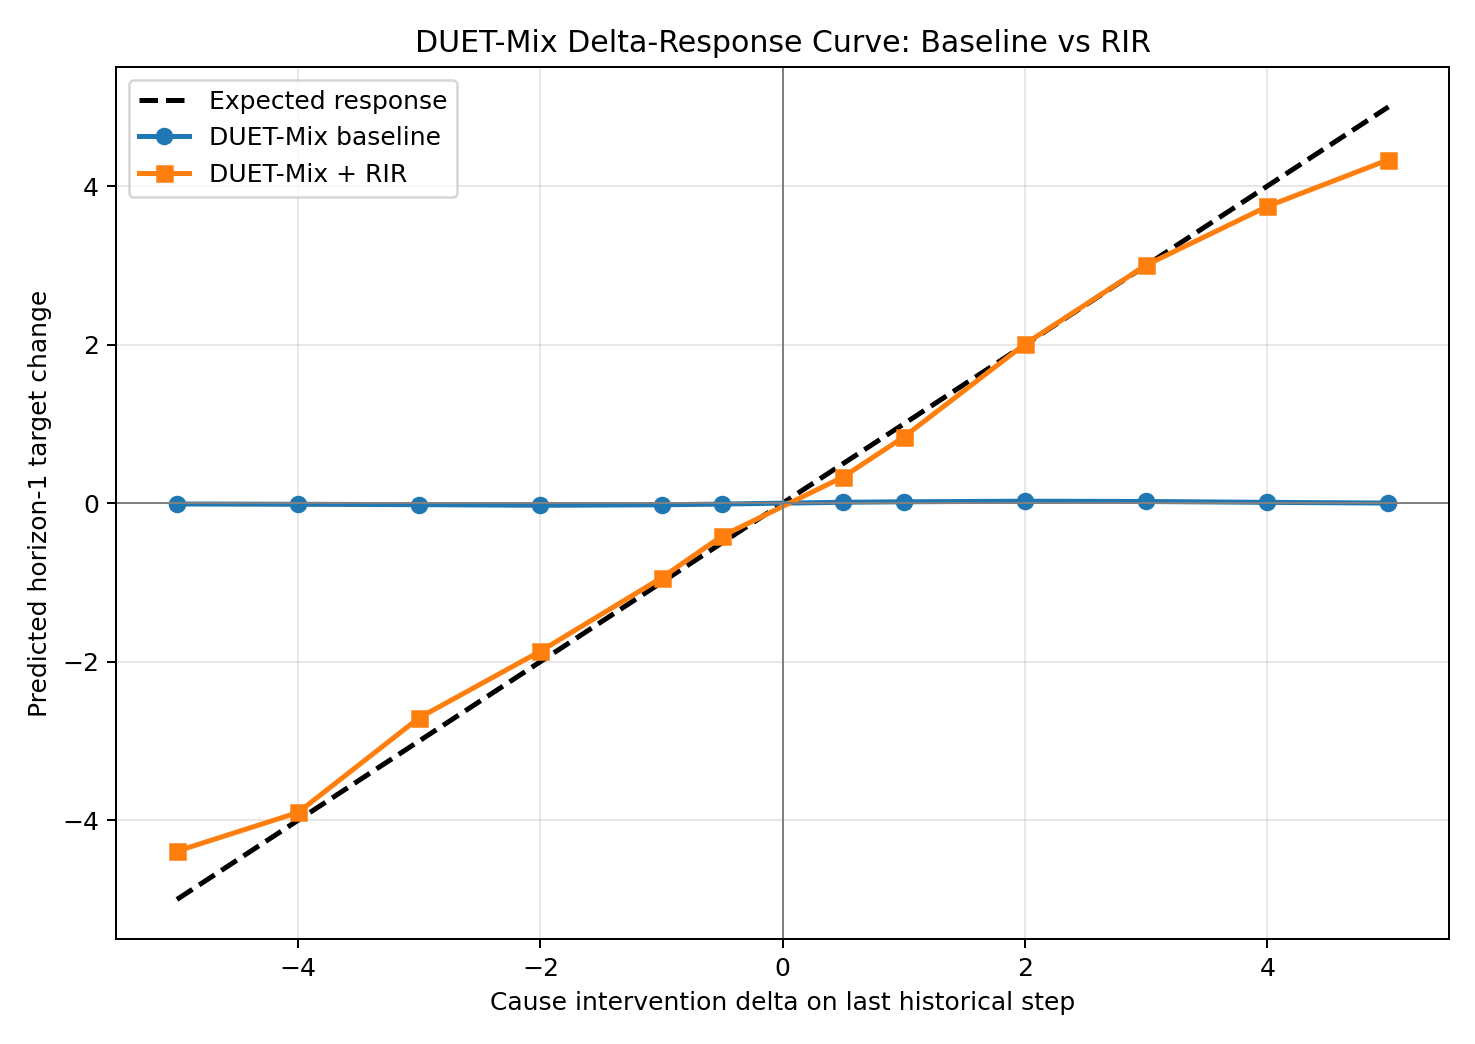
\includegraphics[width=0.72\linewidth]{../results/duet_crr_20260503/duet_baseline_vs_rir_curve.png}
\caption{DUET-Mix delta-response curves. The baseline is nearly flat, while RIR
tracks the analytically expected intervention-response function.}
\label{fig:app_duet_response_curve}
\end{figure}

The DUET-CI + RIR diagnostic should not be interpreted as evidence that a strictly
channel-independent function can use another channel at inference. The inspected
DUET implementation contains shared training components and auxiliary mechanisms,
so response supervision can still alter the learned predictor. We therefore use
DLinear and PatchTST as stricter channel-independent negative controls.

\section{Augmented ETTh1 Details}
\label{app:etth}

For ETTh1 augmented runs, RIR is applied only to the appended semi-synthetic target
and uses $(\lambda_1,\lambda_2)=(0.05,0.005)$. The original \texttt{OT} channel is
never given a response label.

\begin{table}[htbp]
\centering
\caption{Full ETTh1 augmented side-effect diagnostic. Prediction length 96 uses
three seeds; prediction length 192 is a one-seed probe.}
\label{tab:app_etth}
\resizebox{\linewidth}{!}{
\begin{tabular}{llrrrrrr}
\toprule
Pred. len & Variant & All MSE & Raw OT MSE & Raw OT MAE & Semi MSE & Curve slope & Curve IRE \\
\midrule
96 & Baseline & $0.4267{\pm}0.0022$ & $0.0559{\pm}0.0002$ & $0.1828{\pm}0.0004$ & $0.7144{\pm}0.0039$ & $0.0226{\pm}0.0023$ & $2.4149{\pm}0.0056$ \\
96 & + RIR & $0.4265{\pm}0.0043$ & $0.0557{\pm}0.0005$ & $0.1817{\pm}0.0007$ & $0.7078{\pm}0.0083$ & $0.9292{\pm}0.0121$ & $0.3317{\pm}0.0057$ \\
192 & Baseline & $0.4906$ & $0.0728$ & $0.2081$ & $0.8375$ & $0.0147$ & $2.4349$ \\
192 & + RIR & $0.4838$ & $0.0728$ & $0.2071$ & $0.8220$ & $0.9531$ & $0.3082$ \\
\bottomrule
\end{tabular}
}
\end{table}

\section{Augmented ETTh2 Generalization Diagnostic}
\label{app:etth2}

To check whether the augmented-real diagnostic is specific to ETTh1, we repeat the
same construction on ETTh2. We retain the original ETTh2 channels, append
$Y^{\mathrm{rir}}_t=2\cdot\mathrm{HUFL}_{t-1}+s(t)+\epsilon_t$, and apply RIR only
to the appended target. Table~\ref{tab:app_etth2} shows that the baseline response
again collapses near zero, while RIR recovers an almost calibrated response curve.
Unlike the ETTh1 result, raw \texttt{OT} error is modestly higher under RIR on
ETTh2. We therefore treat this experiment as a generalization diagnostic for
response repair, not as evidence that response supervision is always free of
collateral effects on unrelated raw targets.

\begin{table}[htbp]
\centering
\caption{Augmented ETTh2 diagnostic at prediction length 96, reported as mean
$\pm$ standard deviation over three seeds. RIR repairs the appended target's
response curve; raw \texttt{OT} metrics are side-effect diagnostics and are not
causal evidence.}
\label{tab:app_etth2}
\resizebox{\linewidth}{!}{
\begin{tabular}{lrrrrrrr}
\toprule
Variant & All MSE & Raw OT MSE & Raw OT MAE & Semi MSE & Curve slope & Curve IRE & Curve ratio \\
\midrule
Baseline & $0.3217{\pm}0.0021$ & $0.1475{\pm}0.0014$ & $0.2959{\pm}0.0014$ & $0.4788{\pm}0.0050$ & $0.0083{\pm}0.0028$ & $2.5959{\pm}0.0077$ & $0.0100{\pm}0.0032$ \\
+ RIR & $0.3245{\pm}0.0061$ & $0.1607{\pm}0.0049$ & $0.3095{\pm}0.0055$ & $0.4710{\pm}0.0069$ & $1.0033{\pm}0.0215$ & $0.5288{\pm}0.0151$ & $0.8987{\pm}0.0103$ \\
\bottomrule
\end{tabular}
}
\end{table}

\clearpage
\input{checklist}

\end{document}
